\documentclass[11pt,oneside]{article}	%use"amsart"insteadof"article"forAMSLaTeXformat
\usepackage{geometry}		%Seegeometry.pdftolearnthelayoutoptions.Therearelots.
\geometry{letterpaper}		%...ora4paperora5paperor...
%\geometry{landscape}		%Activateforforrotatedpagegeometry
%\usepackage[parfill]{parskip}		%Activatetobeginparagraphswithanemptylineratherthananindent
\usepackage{graphicx}				%Usepdf,png,jpg,orepsßwithpdflatex;useepsinDVImode
								%TeXwillautomaticallyconverteps-->pdfinpdflatex		
\usepackage{amssymb}
\usepackage{amsmath}
\usepackage[colorlinks]{hyperref}

%----macros begin---------------------------------------------------------------
\usepackage{color}
\usepackage{amsthm}
\usepackage{amsmath}

\def\conv{\mbox{\textrm{conv}\,}}
\def\aff{\mbox{\textrm{aff}\,}}
\def\E{\mathbb{E}}
\def\R{\mathbb{R}}
\def\Z{\mathbb{Z}}
\def\tex{\TeX}
\def\latex{\LaTeX}
\def\v#1{{\bf #1}}
\def\p#1{{\bf #1}}
\def\T#1{{\bf #1}}

\def\vet#1{{\left(\begin{array}{cccccccccccccccccccc}#1\end{array}\right)}}
\def\mat#1{{\left(\begin{array}{cccccccccccccccccccc}#1\end{array}\right)}}

\def\lin{\mbox{\rm lin}\,}
\def\aff{\mbox{\rm aff}\,}
\def\pos{\mbox{\rm pos}\,}
\def\cone{\mbox{\rm cone}\,}
\def\conv{\mbox{\rm conv}\,}
\newcommand{\homog}[0]{\mbox{\rm homog}\,}
\newcommand{\relint}[0]{\mbox{\rm relint}\,}

%----macros end-----------------------------------------------------------------

\title{Boolean combinations of cellular complexes as chain operations
\footnote{This document is part of the \emph{Linear Algebraic Representation with CoChains} (LAR-CC) framework~\cite{cclar-proj:2013:00}. \today}
}
\author{Alberto Paoluzzi}
%\date{}							%Activatetodisplayagivendateornodate

\begin{document}
\maketitle
\tableofcontents
\nonstopmode

\section{Introduction}

In this module a novel approach to Boolean operations of cellular complexes is defined and implemented. The novel algorithm may be summarised as follows. 

First we compute the CDC (Common Delaunay Complex) of the input LAR complexes $A$ and $B$, to get a LAR of the \emph{simplicial} CDC.

Then, we split the cells intersecting the boundary faces of the input complexes, getting the final \emph{polytopal} SCDC  
(Split Common Delaunay Complex), whose cells  provide the  basis for the linear coordinate representation of both input 
complexes, upon the same space decomposition.

Finally, every Boolean result is computed by bitwise operations, between the coordinate representations of the transformed 
$A$ and $B$ input.



\subsection{Preview of the Boolean algorithm}

The goal is the computation of $A \diamond B$, with $\diamond\in \{\cup, \cap, -\}$, where a LAR representation of both $A$ and $B$ is given. The Boolean algorithm works as follows.

\begin{enumerate}
\item 
Embed both cellular complexes $A$ and $B$ in the same space (say, identify their common vertices) by $V_{ab} = V_a \cup V_b$.
\item 
Build their CDC  (Common Delaunay Complex) as the LAR of \emph{Delaunay triangulation} of the vertex set $V_{ab}$.
\item 
Split the (highest-dimensional) cells of CDC crossed by $\partial A$ or $\partial B$. Their lower dimensional faces remain partitioned accordingly. We name the resulting complex SCDC (Split Common Delaunay Complex).
\item 
With respect to the SCDC basis of $d$-cells $C_d$, compute two coordinate chains $\alpha,\beta: C_d \to \{0,1\}$, such that: 
\begin{align}
	\alpha(cell) &= 1  \quad\mbox{if\ } |cell| \subset A;  \quad\mbox{else\ } \alpha(cell) = 0, \nonumber\\
	\beta(cell) &= 1  \quad\mbox{if\ } |cell| \subset B;  \quad\mbox{else\ } \beta(cell) = 0. \nonumber
\end{align}
\item 
Extract accordingly the SCDC chain corresponding to $A \diamond B$, with $\diamond\in \{\cup, \cap, -\}$.
\end{enumerate}


\subsubsection{Remarks}
You may  make an analogy between the SCDC (\emph{Split} CDC) and a CDT (Constrained Delaunay Triangulation).  In part they coincide, but in general, the SCDC is a polytopal complex, and is not a simplicial complex as the CDC.

The more complex algorithmic step is the cell splitting.  
Every time, a single $d$-cell  $c$  is split by a single hyperplane (cutting its interior)  giving either two splitted cells $c_1$ and $c_2$, or just one output cell (if the hyperplane is the affine hull of the CDC facet)
whatever the input cell dimension $d$.  After every splitting of the cell interior, the row $c$ is substituted (within the \texttt{CV} matrix) by $c_1$, and $c_2$ is 
added to the end of the \texttt{CV} matrix, as a new row.

The splitting process is started by ``splitting seeds" generated by $(d-1)$-faces of both operand boundaries.
In fact, every such face, say $f$, has vertices on CDC and \emph{may} split some incident CDC $d$-cell.  In particular, starting from its vertices,
$f$ must split the CDC cells in whose interior it passes though.

So, a dynamic data structure is set-up, storing for each boundary face $f$ the list of cells it must cut, and, for every CDC $d$-cell with interior traversed
by some such $f$, the list of cutting faces.  This data structure is continuously updated during the splitting process, using the 
adjacent cells of the split ones, who are to be split in turn.  Every split cell may add some adjacent cell to be split, and after the split,
the used pair (\texttt{cell,face}) is removed.  The splitting process continues until the data structure becomes empty.

Every time a cell is split, it is characterized as either internal (1) or external (0) to the used (oriented) boundary facet f, so that the two 
resulting subcells $c_1$ and $c_2$  receive two opposite characterization (with respect to the considered boundary).

At the very end, every (polytopal) SCDC $d$-cell has two bits of information (one for argument $A$ and one for argument $B$), telling whether it is internal  (1) or external (0) or unknown (-1) with respect to every Boolean argument.

A final recursive traversal of the SCDC, based on cell adjacencies, transforms every $-1$ into either 0 or 1, providing the two final chains to be bitwise operated, depending on the Boolean operation to execute.


\section{Merging arguments}

%-------------------------------------------------------------------------------
\subsection{Reordering of vertex coordinates}
%-------------------------------------------------------------------------------
A global reordering of vertex coordinates is executed as the first step of the Boolean algorithm, in order to eliminate the duplicate vertices, by substituting duplicate vertex copies (coming from two close points) with a single instance. 

Two dictionaries are created, then merged in a single dictionary, and finally split into three subsets of (vertex,index) pairs, with the aim of rebuilding the input representations, by making use of a novel and more useful vertex indexing.

The union set of vertices is finally reordered using the three subsets of vertices belonging (a) only to the first argument, (b) only to the second argument and (c) to both, respectively denoted as $V_1, V_2, V_{12}$. A top-down description of this initial computational step is provided by the set of macros discussed in this section.

%-------------------------------------------------------------------------------
@D Place the vertices of Boolean arguments in a common space
@{""" First step of Boolean Algorithm """
@< Initial indexing of vertex positions @>
@< Merge two dictionaries with keys the point locations @>
@< Filter the common dictionary into three subsets @>
@< Compute an inverted index to reorder the vertices of Boolean arguments @>
@< Return the single reordered pointset and the two $d$-cell arrays @>
@}
%-------------------------------------------------------------------------------

%-------------------------------------------------------------------------------
\subsubsection{Re-indexing of vertices}
%-------------------------------------------------------------------------------

\paragraph{Initial indexing of vertex positions}
The input LAR models are located in a common space by (implicitly) joining \texttt{V1} and \texttt{V2} in a same array, and (explicitly) shifting the vertex indices in \texttt{CV2} by the length of \texttt{V1}.
%-------------------------------------------------------------------------------
@D Initial indexing of vertex positions
@{from collections import defaultdict, OrderedDict

""" TODO: change defaultdict to OrderedDefaultdict """

class OrderedDefaultdict(collections.OrderedDict):
    def __init__(self, *args, **kwargs):
        if not args:
            self.default_factory = None
        else:
            if not (args[0] is None or callable(args[0])):
                raise TypeError('first argument must be callable or None')
            self.default_factory = args[0]
            args = args[1:]
        super(OrderedDefaultdict, self).__init__(*args, **kwargs)

    def __missing__ (self, key):
        if self.default_factory is None:
            raise KeyError(key)
        self[key] = default = self.default_factory()
        return default

    def __reduce__(self):  # optional, for pickle support
        args = (self.default_factory,) if self.default_factory else tuple()
        return self.__class__, args, None, None, self.iteritems()


def vertexSieve(model1, model2):
	from lar2psm import larModelBreak
	V1,CV1 = larModelBreak(model1) 
	V2,CV2 = larModelBreak(model2)
	n = len(V1); m = len(V2)
	def shift(CV, n): 
		return [[v+n for v in cell] for cell in CV]
	CV2 = shift(CV2,n)
@}
%-------------------------------------------------------------------------------

\paragraph{Merge two dictionaries with point location as keys}
Since currently \texttt{CV1} and \texttt{CV2} point to a set of vertices larger than their initial sets 
\texttt{V1} and \texttt{V2}, we re-index the set $\texttt{V1} \cup \texttt{V2}$ using a Python \texttt{defaultdict} dictionary, in order to avoid errors of ``missing key". As dictionary keys, we use the string representation of the vertex position vector, with a given fixed floating-point approximation, as provided by the \texttt{vcode} function discussed in the in the Appendix of this document.
%-------------------------------------------------------------------------------
@D Merge two dictionaries with keys the point locations
@{	
	vdict1 = defaultdict(list)
	for k,v in enumerate(V1): vdict1[vcode(v)].append(k) 
	vdict2 = defaultdict(list)
	for k,v in enumerate(V2): vdict2[vcode(v)].append(k+n) 
	
	vertdict = defaultdict(list)
	for point in vdict1.keys(): vertdict[point] += vdict1[point]
	for point in vdict2.keys(): vertdict[point] += vdict2[point]
@}
%-------------------------------------------------------------------------------

\paragraph{Example of string coding of a vertex position}
The position vector of a point of real coordinates is provided by the function \texttt{vcode}.
An example of coding is given below. The \emph{precision} of the string representation can be tuned at will.
{\small
\begin{verbatim}
>>> vcode([-0.011660381062724849, 0.297350056848685860])
'[-0.0116604, 0.2973501]'
\end{verbatim}}



\paragraph{Filter the common dictionary into three subsets}
\texttt{Vertdict}, dictionary of vertices, uses as key the position vectors of vertices coded as string, and as values the list of integer indices of vertices on the given position. If the point position belongs either to the first or to second argument only, it is stored in \texttt{case1} or \texttt{case2} lists respectively. If the position (\texttt{item.key}) is shared between two vertices, it is stored in \texttt{case12}.
The variables \texttt{n1}, \texttt{n2}, and \texttt{n12} remember the number of vertices respectively stored in each repository.
%-------------------------------------------------------------------------------
@D Filter the common dictionary into three subsets
@{	
	case1, case12, case2 = [],[],[]
	for item in vertdict.items():
		key,val = item
		if len(val)==2:  case12 += [item]
		elif val[0] < n: case1 += [item]
		else: case2 += [item]
	n1 = len(case1); n2 = len(case12); n3 = len(case2)
@}
%-------------------------------------------------------------------------------

\paragraph{Compute an inverted index to reorder the vertices of Boolean arguments}
The new indices of vertices are computed according with their position within the storage repositories \texttt{case1}, \texttt{case2}, and \texttt{case12}. Notice that every \texttt{item[1]} stored in \texttt{case1} or \texttt{case2} is a list with only one integer member. Two such values are conversely stored in each \texttt{item[1]} within \texttt{case12}.
%-------------------------------------------------------------------------------
@D Compute an inverted index to reorder the vertices of Boolean arguments 
@{
	invertedindex = list(0 for k in range(n+m))
	for k,item in enumerate(case1):
		invertedindex[item[1][0]] = k
	for k,item in enumerate(case12):
		invertedindex[item[1][0]] = k+n1
		invertedindex[item[1][1]] = k+n1
	for k,item in enumerate(case2):
		invertedindex[item[1][0]] = k+n1+n2
@}
%-------------------------------------------------------------------------------

%-------------------------------------------------------------------------------
\subsubsection{Re-indexing of d-cells}
%-------------------------------------------------------------------------------

\paragraph{Return the single reordered pointset and the two $d$-cell arrays}
We are now finally ready to return two reordered LAR models defined over the same set \texttt{V} of vertices, and where (a) the vertex array \texttt{V} can be written as the union of three disjoint sets of points $C_1,C_{12},C_2$; (b) the $d$-cell array \texttt{CV1} is indexed over $C_1\cup C_{12}$; (b) the $d$-cell array \texttt{CV2} is indexed over $C_{12}\cup C_{2}$. 

The \texttt{vertexSieve} function will return the new reordered vertex set $V = (V_1 \cup V_2) \setminus (V_1 \cap V_2)$, the two renumbered $s$-cell sets \texttt{CV1} and \texttt{CV2}, and the size \texttt{len(case12)} of $V_1 \cap V_2$.
%-------------------------------------------------------------------------------
@D Return the single reordered pointset and the two $d$-cell arrays
@{
	V = [eval(p[0]) for p in case1] + [eval(p[0]) for p in case12] + [eval(
				p[0]) for p in case2]
	CV1 = [sorted([invertedindex[v] for v in cell]) for cell in CV1]
	CV2 = [sorted([invertedindex[v] for v in cell]) for cell in CV2]
	return V, CV1, CV2, len(case12)
@}
%-------------------------------------------------------------------------------


\subsubsection{Example of input with some coincident vertices}
In this example we give two very simple LAR representations of 2D cell complexes, with some coincident vertices, and go ahead to re-index the vertices, according to the method implemented by the function \texttt{vertexSieve}.

%-------------------------------------------------------------------------------
@o test/py/bool/test02.py
@{@< Initial import of modules @>
from bool import *
V1 = [[1,1],[3,3],[3,1],[2,3],[2,1],[1,3]]
V2 = [[1,1],[1,3],[2,3],[2,2],[3,2],[0,1],[0,0],[2,0],[3,0]]
CV1 = [[0,3,4,5],[1,2,3,4]]
CV2 = [[3,4,7,8],[0,1,2,3,5,6,7]]
model1 = V1,CV1; model2 = V2,CV2
VIEW(STRUCT([ 
	COLOR(CYAN)(SKEL_1(STRUCT(MKPOLS(model1)))), 
	COLOR(RED)(SKEL_1(STRUCT(MKPOLS(model2)))) ]))
@}
%-------------------------------------------------------------------------------

\paragraph{Example discussion} 
The aim of the \texttt{vertexSieve} function is twofold: (a) eliminate vertex duplicates before entering the main part of the Boolean algorithm; (b) reorder the input representations so that it becomes less expensive to check whether a 0-cell can be shared by both the arguments of a Boolean expression, so that its coboundaries must be eventually split. Remind that for any set it is:
\[
|A\cup B| = |A|+|B|-|A\cap B|.
\]
Let us notice that in the previous example
\[
|V| = |V_1 \cup V_2| = 12 \leq |V_1|+|V_2| = 6+9 = 15,
\]
and that 
\[
|V_1|+|V_2| - |V_1 \cup V_2| = 15 - 12 = 3 = |C_{12}| = |V_1 \cap V_2|,
\]
where $C_{12}$ is the subset of vertices with duplicated instances.
%-------------------------------------------------------------------------------
@D Output from \texttt{test/py/boolean/test02.py}
@{V   = [[3.0,1.0],[2.0,1.0],[3.0,3.0],[1.0,1.0],[1.0,3.0],[2.0,3.0],
		 [3.0,2.0],[2.0,0.0],[2.0,2.0],[0.0,0.0],[3.0,0.0],[0.0,1.0]]
CV1 = [[3,5,1,4],[2,0,5,1]]
CV2 = [[8,6,7,10],[3,4,5,8,11,9,7]]
@}
%-------------------------------------------------------------------------------
Notice also that \texttt{V} has been reordered in three consecutive subsets $C_{1},C_{12},C_{2}$ such that \texttt{CV1} is indexed within $C_{1}\cup C_{12}$, whereas \texttt{CV2} is indexed within $C_{12}\cup C_{2}$. In our example we have  $C_{12}=\{\texttt{3,4,5}\}$: 
%-------------------------------------------------------------------------------
@D Reordering of vertex indexing of cells
@{
>>> sorted(CAT(CV1))
[0, 1, 1, 2, 3, 4, 5, 5]
>>> sorted(CAT(CV2))
[3, 4, 5, 6, 7, 7, 8, 8, 9, 10, 11]
@}
%-------------------------------------------------------------------------------
\paragraph{Cost analysis} 
Of course, this reordering after elimination of duplicate vertices will allow to perform a cheap $O(n)$ discovering of (Delaunay) cells whose vertices belong both to \texttt{V1} \emph{and} to \texttt{V2}. 
Actually, the \emph{same test} can be now used both when the vertices of the input arguments are all different, \emph{and} when they have some coincident vertices.
The total cost of such pre-processing, executed using dictionaries, is $O(n\ln n)$.

%-------------------------------------------------------------------------------

\subsubsection{Example}

\paragraph{Building a covering of Common Delaunay Complex}

%-------------------------------------------------------------------------------
@D Building a covering of Common Delaunay Complex
@{def covering(model1,model2,dim=2,emptyCellNumber=1):
	V, CV1, CV2, n12 = vertexSieve(model1,model2)
	_,EEV1 = larFacets((V,CV1),dim,emptyCellNumber)
	_,EEV2 = larFacets((V,CV2),dim,emptyCellNumber)
	if emptyCellNumber !=0: CV1 = CV1[:-emptyCellNumber]
	if emptyCellNumber !=0: CV2 = CV2[:-emptyCellNumber]
	VV = AA(LIST)(range(len(V)))
	return V,[VV,EEV1,EEV2,CV1,CV2],n12
@}
%-------------------------------------------------------------------------------

\begin{figure}[htbp] %  figure placement: here, top, bottom, or page
   \centering
   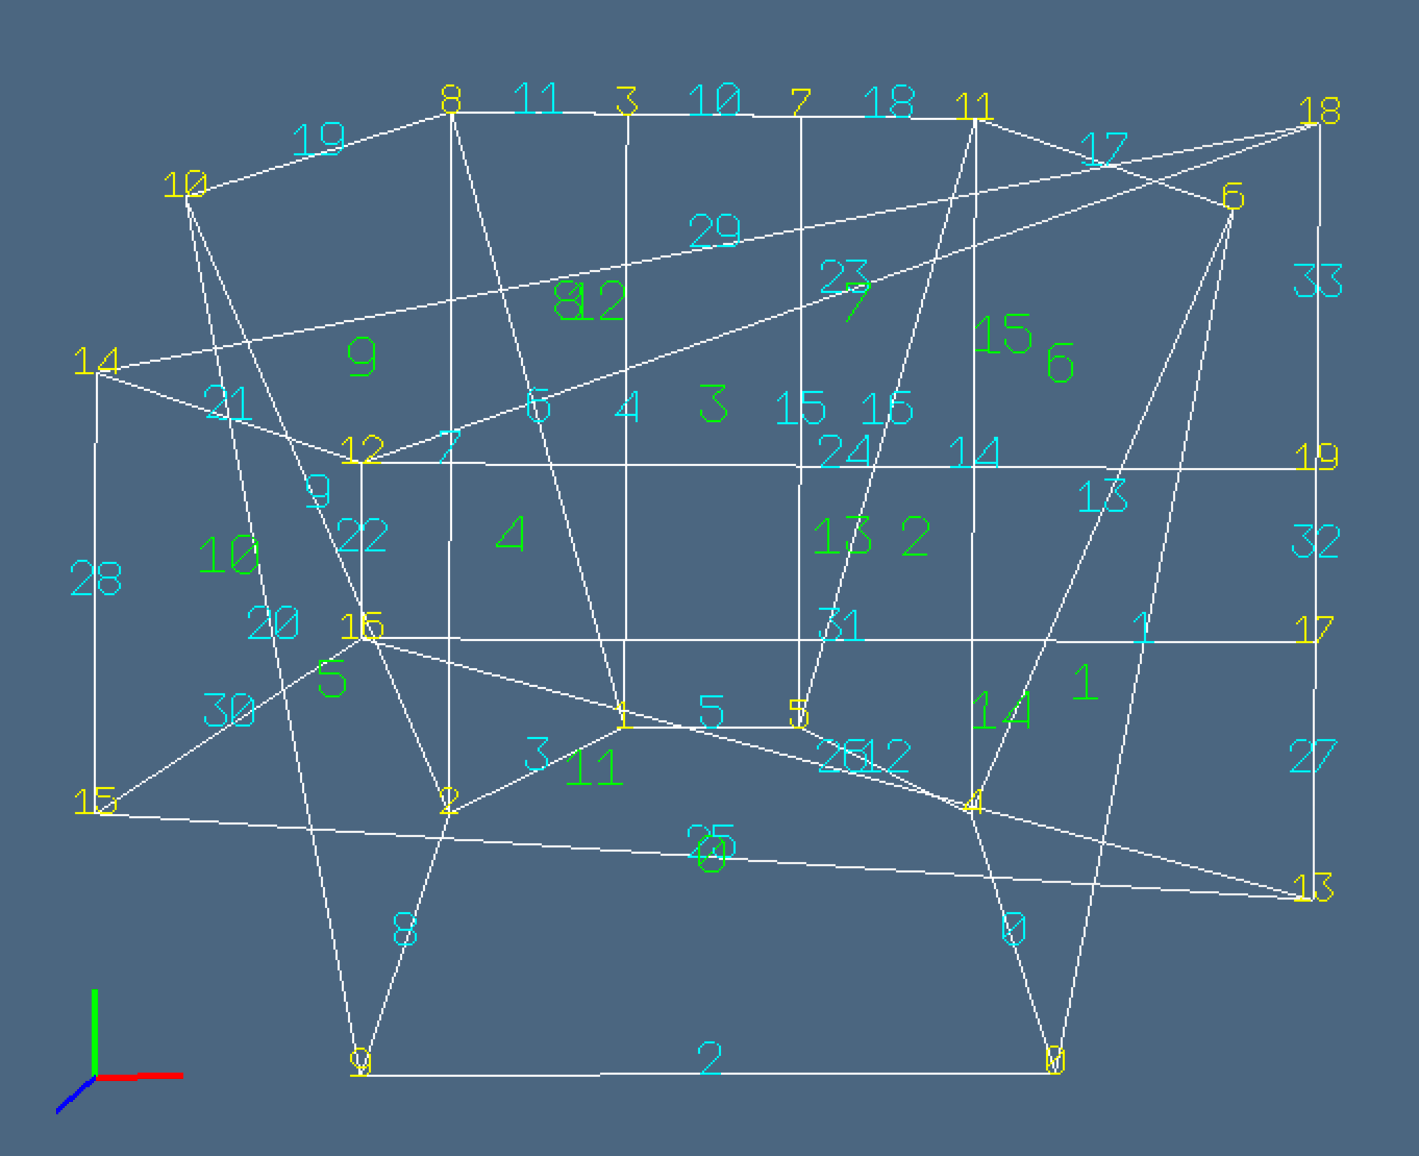
\includegraphics[width=0.6\linewidth]{images/covering} 
   \caption{Set covering of the two Boolean arguments.}
   \label{fig:example}
\end{figure}




\section{Selecting cells to split}

The aim of this section is to provide some fast method to select a subset of CDC cells where to start the 
splitting of the CDC along the $(d-1)$ boundary facets of operand complexes. Of course,  a lot of useful information is provided  by the incidence relation \texttt{VC} between CDC vertices and $d$-cells. 

Two dictionaries are used in order to split the CDC and compute the SCDC. The dictionary \texttt{dict\_fc} is used with key a boundary $(d-1)$-face and value the (dynamic) list of CDC $d$-cells crossed (and later split) by it. Conversely, the  \texttt{dict\_cf} dictionary is used with key a CDC $d$-cell and with value the list of boundary $(d-1)$-faces crossing it.

Two different strategies may be used for boundary facets terminating by crossing the interior of some CDC cell, and for facets sharing the tangent space of the boundary of such cells.
Alternatively to what initially implemented, all the boundary $(d-1)$-faces must be considered as ``splitting seeds", and tracked against the current state of the SCDC.


\paragraph{Relational inversion (characteristic matrix transposition)}

The operation could be executed by simple matrix transposition of the CSR (Compressed Sparse Row) representation of the sparse characteristic matrix $M_d \equiv \texttt{CV}$.
A simple relational inversion using Python lists is given here. The \texttt{invertRelation} function 
is given here, linear in the size of the \texttt{CV} list, where the complexity of each cell is constant and 
small in most cases.

%-------------------------------------------------------------------------------
@D Characteristic matrix transposition
@{""" Characteristic matrix transposition """
def invertRelation(V,CV):
	VC = [[] for k in range(len(V))]
	for k,cell in enumerate(CV):
		for v in cell:
			VC[v] += [k]
	return VC
@}
%-------------------------------------------------------------------------------


\subsection{Computing the boundary hyperplanes (BHs)}

For each boundary $(d-1)$-face the affine hull is computed, producing a set of pairs (\texttt{face, covector}).

%-------------------------------------------------------------------------------
@D New implementation of splitting dictionaries
@{""" New implementation of splitting dictionaries """
VC = invertRelation(V,CV)

covectors = []
for faceVerts in BC:
	points = [V[v] for v in faceVerts]
	dim = len(points[0])
	theMat = Matrix( [(dim+1)*[1.]] + [p+[1.] for p in points] )
	covector = [(-1)**(col)*theMat.minor(0,col).determinant() 
						for col in range(dim+1)]
	covectors += [covector]

@< Association of covectors to d-cells @>
@< Initialization of splitting dictionaries @>
@}
%-------------------------------------------------------------------------------



\subsection{Association of BHs to $d$-cells of CDC}

Every pair (\texttt{face, covector}) is associated uniquely to a single $d$-cell of CDC, producing a set of triples (\texttt{face, covector, cell}). Two cases are possible: (a) the face hyperplane crosses the interior of the cell; (b) the face hyperplane contains the face, so that the cell is left on the interior subspace of the (oriented) face covector.

For this purpose, it is checked that at least one of the face vertices, transformed into the common-vertex-based coordinate frame, have all positive coordinates. This fact guarantees the existence of a non trivial intersection between the $(d-1)$-face and the $d$-cell.


%-------------------------------------------------------------------------------
@D Association of covectors to d-cells
@{""" to compute a single d-cell associated to (face,covector) """
def covectorCell(face,faceVerts,covector,CV,VC):
	incidentCells = VC[faceVerts[0]]
	for cell in incidentCells:
		cellVerts = CV[cell]
		v0 = list(set(faceVerts).intersection(cellVerts))[0] # v0 = common vertex
		transformMat = mat([DIFF([V[v],V[v0]]) for v in cellVerts if v != v0]).T.I
		vects = (transformMat * (mat([DIFF([V[v],V[v0]]) for v in faceVerts 
					if v != v0]).T)).T.tolist()
		if any([all([x>=-0.0001 for x in list(vect)]) for vect in vects]): 
			return [face,cell,covector]
	print "error: found no face,cell,covector","\n"
@}
%-------------------------------------------------------------------------------




\subsection{Initialization of splitting dictionaries}
The triples (\texttt{face, cell, covector}), computed by the \texttt{covectorCell} function, is suitably accommodated into two dictionaries denoted as \texttt{dict\_fc} (for \emph{face, cell}) and \texttt{dict\_cf} (for \emph{cell, face}), respectively.


%-------------------------------------------------------------------------------
@D Initialization of splitting dictionaries
@{""" Initialization of splitting dictionaries """
tasks = []
for face,covector in zip(range(len(BC)),covectors):
	tasks += [covectorCell(face,BC[face],covector,CV,VC)]

dict_fc,dict_cf = initTasks(tasks)
print "\n>dict_cf",dict_cf
print "\n>dict_fc",dict_fc,"\n"
@}
%-------------------------------------------------------------------------------



\section{Splitting cells traversing the boundaries}
\label{sec:crossing}
In the previous section we computed a set of "split seeds", each made by a boundary facet and by a Delaunay cell to be split by the facet's affine hull. Here we show how to partition ate each such cells into two cells, according to Figure~\ref{fig:splitting}, where the boundary facets of the two boolean arguments are shown in yellow color.

\begin{figure}[htbp] %  figure placement: here, top, bottom, or page
   \centering
   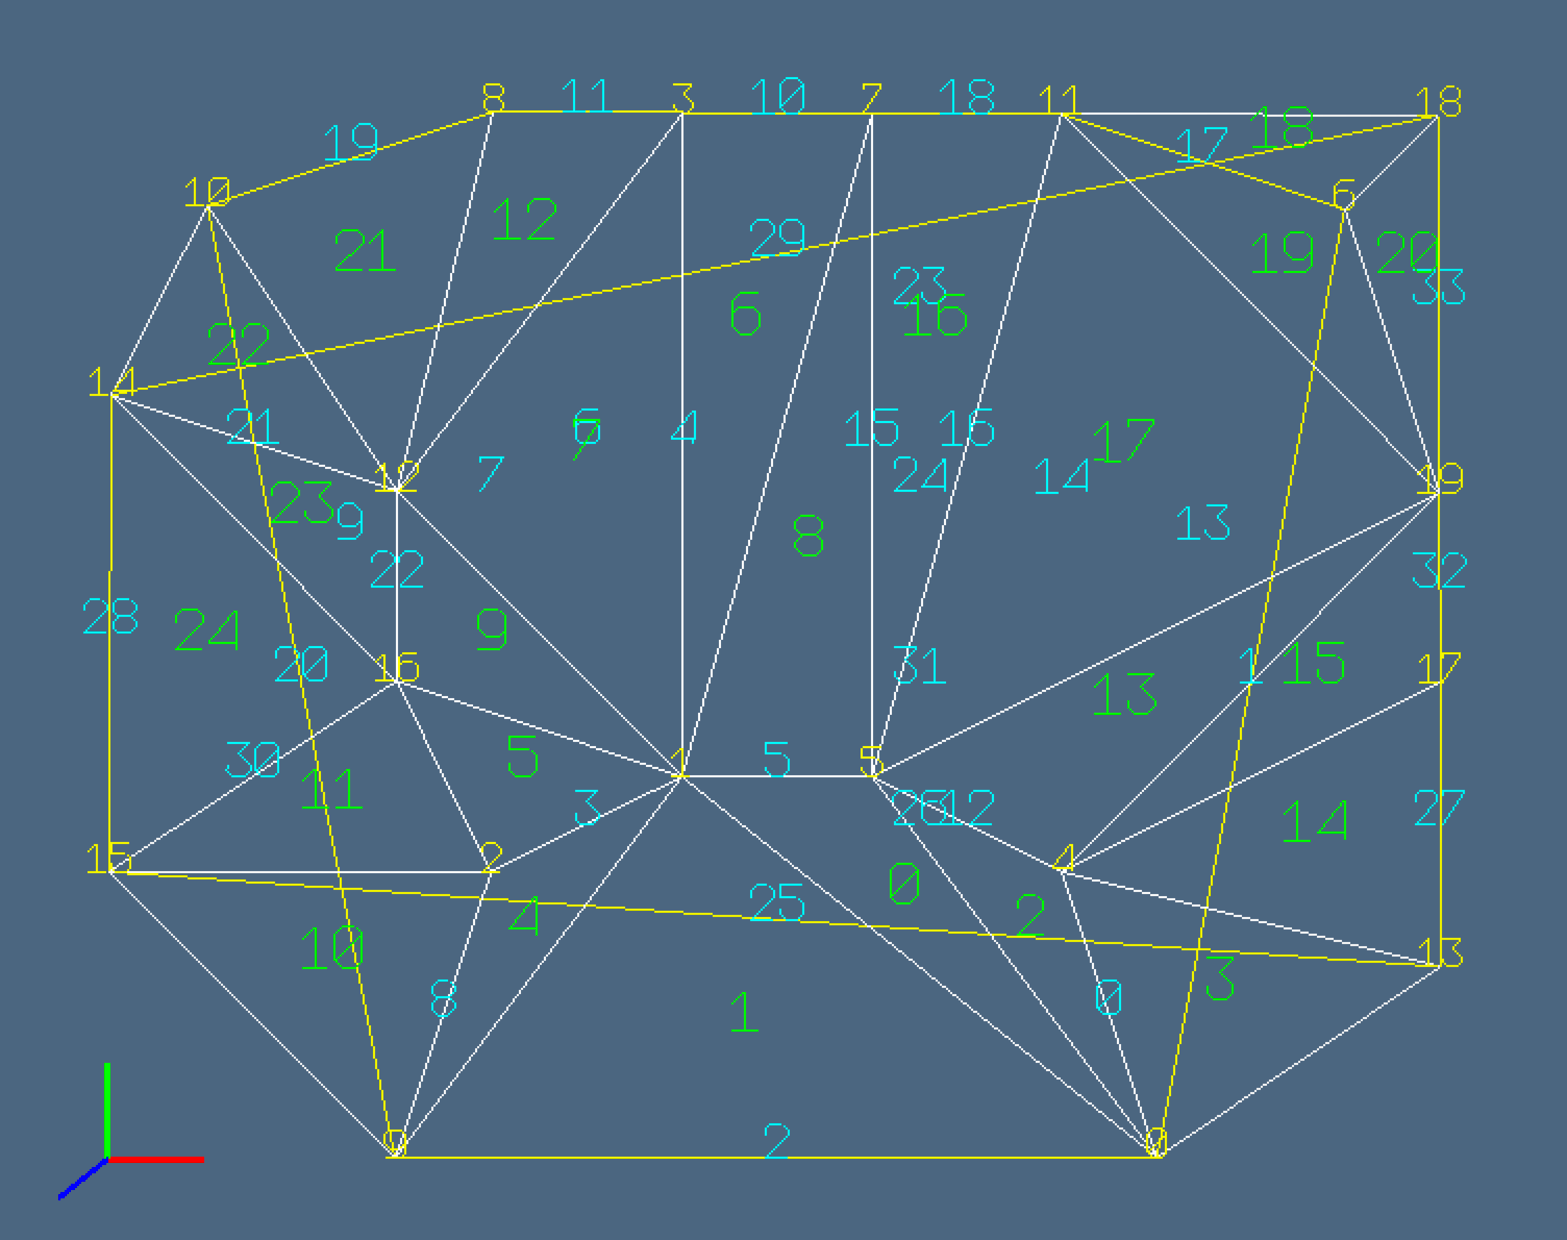
\includegraphics[width=0.6\linewidth]{images/splitting} 
   \caption{example caption}
   \label{fig:splitting}
\end{figure}

In the example in Figure~\ref{fig:splitting}, the set of pairs \texttt{(facet,cell)} to be used as split seeds are given below.
{\small
\begin{verbatim}
[[25, 3], [1, 3], [29, 18], [20, 22], [1, 19], [25, 10], [20, 10], [29, 22]]
\end{verbatim}}

\subsection{Cell splitting}

A cell will be split by pyplasm intersection with a suitable rotated and translated instance of a (large) $d$-cuboid with the superior face embedded in the hyperplane $z=0$.

\paragraph{Splitting a cell with an hyperplane}
The macro below defines a function \texttt{cellSplitting}, with input the index of the \texttt{face}, the index of the \texttt{cell} to be bisected, the \texttt{covector} giving the coefficients of the splitting hyperplane, i.e.~the affine hull of the splitting \texttt{face}, and the arrays \texttt{V}, \texttt{EEV}, \texttt{CV}, giving the coordinates of vertices, the (accumulated) facet to vertices relation (on the input models), and the cell to vertices relation (on the Delaunay model), respectively. 

The actual subdivision of the input \texttt{cell} onto the two output cells \texttt{cell1} and \texttt{cell2} is performed by using the \texttt{pyplasm} Boolean operations of intersection and difference of the input with a solid simulation of the needed hyperspace, provided by the \texttt{rototranslSubspace} variable. Of course, such pyplasm operators return two Hpc values, whose vertices will then extracted using the \texttt{UKPOL} primitive.

%-------------------------------------------------------------------------------
@D Cell splitting
@{""" Cell splitting in two cells """
def cellSplitting(face,cell,covector,V,EEV,CV):

	dim = len(V[0])
	subspace = (T(range(1,dim+1))(dim*[-50])(CUBOID(dim*[100])))
	normal = covector[:-1]
	if len(normal) == 2:  # 2D complex
		rotatedSubspace = R([1,2])(ATAN2(normal)-PI/2)(T(2)(-50)(subspace))
	elif len(normal) == 3:  # 3D complex
		rotatedSubspace = R()()(subspace)
	else: print "rotation error"
	t = V[EEV[face][0]]
	rototranslSubspace = T(range(1,dim+1))(t)(rotatedSubspace)
	cellHpc = MKPOL([V,[[v+1 for v in CV[cell]]],None])
	
	# cell1 = INTERSECTION([cellHpc,rototranslSubspace])
	tolerance=10**-PRECISION
	use_octree=False
	cell1 = Plasm.boolop(BOOL_CODE_AND, 
		[cellHpc,rototranslSubspace],tolerance,plasm_config.maxnumtry(),use_octree)
	verts,cells,pols = UKPOL(cell1)
	cell1 = AA(vcode)(verts)

	# cell2 = DIFFERENCE([cellHpc,rototranslSubspace])	
	cell2 = Plasm.boolop(BOOL_CODE_DIFF, 
		[cellHpc,rototranslSubspace],tolerance,plasm_config.maxnumtry(),use_octree)
	verts,cells,pols = UKPOL(cell2)
	cell2 = AA(vcode)(verts)

	return cell1,cell2
@}
%-------------------------------------------------------------------------------

\begin{figure}[htbp] %  figure placement: here, top, bottom, or page
   \centering
   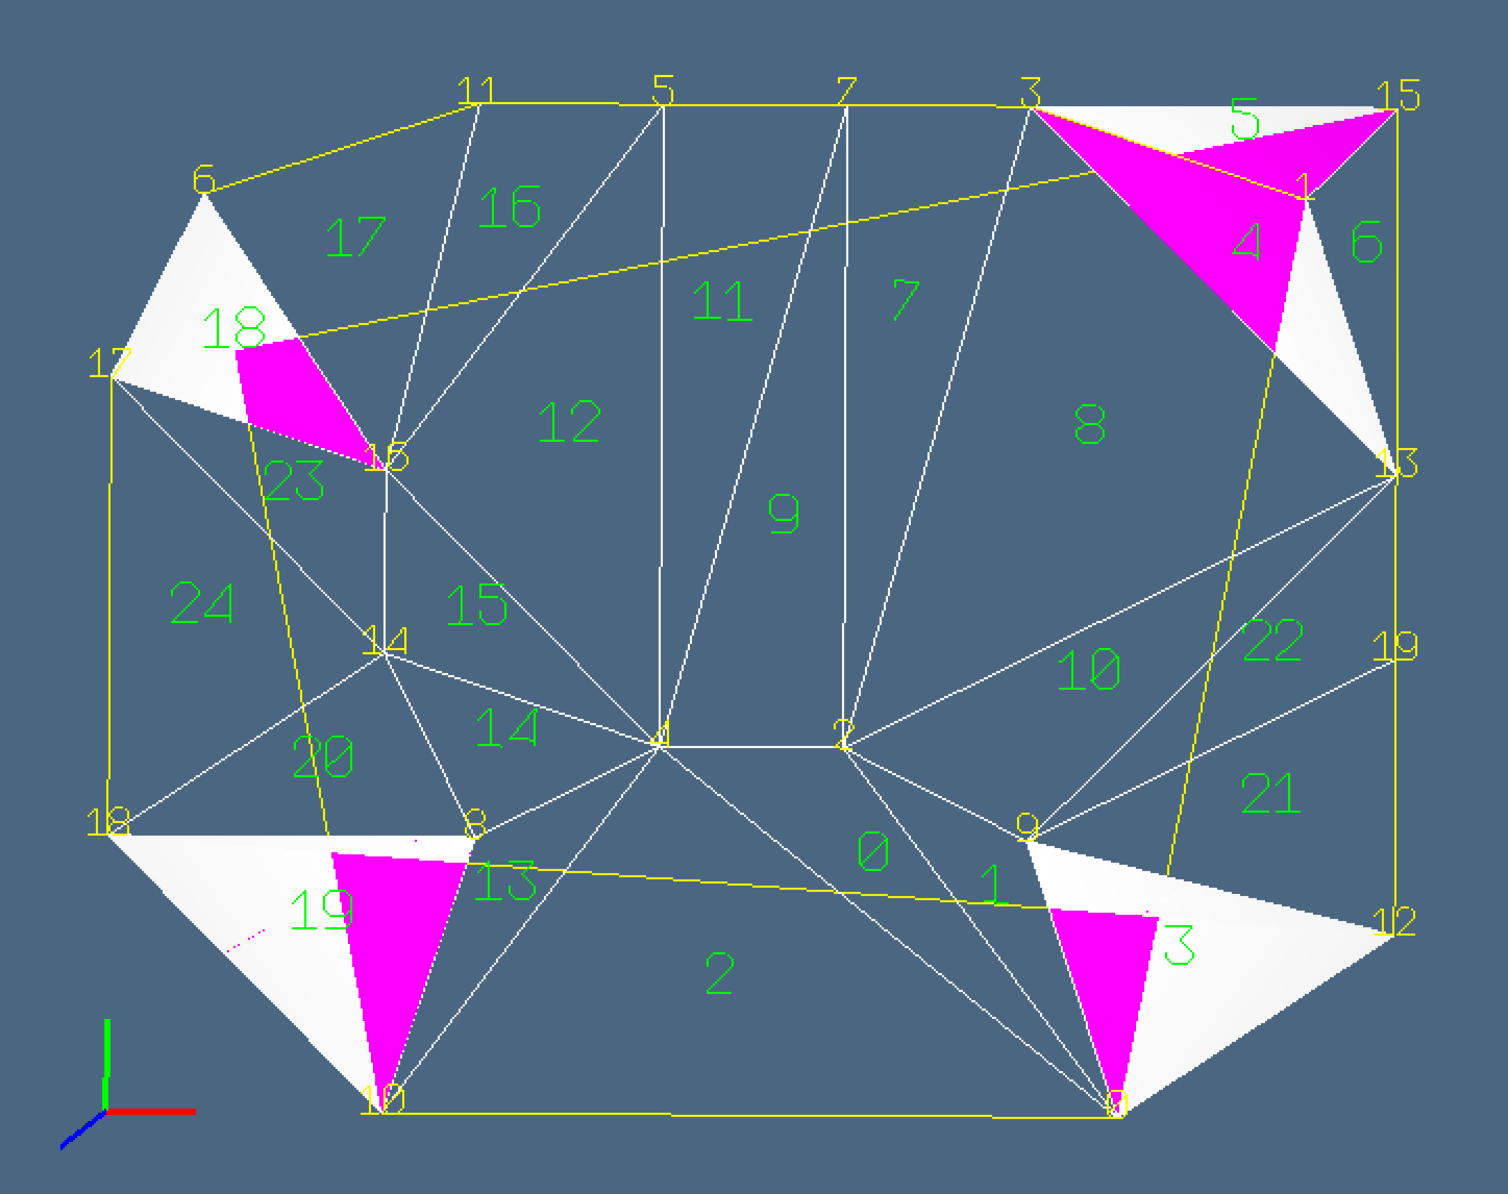
\includegraphics[width=0.6\linewidth]{images/seeds} 
   \caption{example caption}
   \label{fig:example}
\end{figure}


\subsection{Cross-building of two task dictionaries}

The correct and efficient splitting of the Common Delaunay Complex (CDC) with the  (closed and orientable) boundaries of two Boolean arguments, requires the use of two special dictionaries, respectively named \texttt{dict\_fc} (for \emph{face-cell}), and \texttt{dict\_cf} (for \emph{cell-face}).
 
On one side, for each splitting facet ($(d-1)$-face), used as key, we store in \texttt{dict\_fc} the list of traversed $d$-cells of CDC, starting in 2D with the two cells containing the two extreme vertices of the cutting edge, and in higher dimensions, with all the $d$-cells containing one of vertices of the splitting $(d-1)$-face.

On the other side, for each $d$-cell to be split, used as key, we store in \texttt{dict\_cf} the list of cutting $(d-1)$-cells, since a single $d$-cell may be traversed and split by more than one facet. 


\paragraph{Init face-cell and cell-face dictionaries}

%-------------------------------------------------------------------------------
@D Init face-cell and cell-face dictionaries
@{""" Init face-cell and cell-face dictionaries """
def initTasks(tasks):
	dict_fc = defaultdict(list)
	dict_cf = defaultdict(list)
	for task in tasks:
		face,cell,covector = task
		dict_fc[face] += [(cell,covector)] 
		dict_cf[cell] += [(face,covector)] 
	return dict_fc,dict_cf
@}
%-------------------------------------------------------------------------------

\paragraph{Example of face-cell and cell-face dictionaries}

%-------------------------------------------------------------------------------
@D Example of face-cell and cell-face dictionaries
@{""" Example of face-cell and cell-face dictionaries """
tasks (face,cell) = [
 [0, 4, [-10.0, 2.0, 110.0]],
 [31, 5, [3.0, -14.0, 112.0]],
 [17, 18, [10.0, 2.0, -30.0]],
 [22, 3, [-1.0, -14.0, 42.0]],
 [17, 19, [10.0, 2.0, -30.0]],
 [31, 18, [3.0, -14.0, 112.0]],
 [22, 19, [-1.0, -14.0, 42.0]],
 [0, 3, [-10.0, 2.0, 110.0]]]

tasks (dict_fc) = defaultdict(<type 'list'>, {
  0: [(4, [-10.0, 2.0, 110.0]), (3, [-10.0, 2.0, 110.0])],
 17: [(18, [10.0, 2.0, -30.0]), (19, [10.0, 2.0, -30.0])],
 22: [(3, [-1.0, -14.0, 42.0]), (19, [-1.0, -14.0, 42.0])],
 31: [(5, [3.0, -14.0, 112.0]), (18, [3.0, -14.0, 112.0])]  })

tasks (dict_cf) = defaultdict(<type 'list'>, {
 19: [(17, [10.0, 2.0, -30.0]), (22, [-1.0, -14.0, 42.0])],
 18: [(17, [10.0, 2.0, -30.0]), (31, [3.0, -14.0, 112.0])],
  3: [(22, [-1.0, -14.0, 42.0]), (0, [-10.0, 2.0, 110.0])],
  4: [(0, [-10.0, 2.0, 110.0])],
  5: [(31, [3.0, -14.0, 112.0])]  })
@}
%-------------------------------------------------------------------------------


\subsection{Updating the vertex set and dictionary}
\label{sec:updating}

In any dimension, the split of a $d$-cell with an hyperplane (crossing its interior) produces two $d$-cells and some new vertices living upon the splitting hyperplane.

When the $d$-cell $c$ is contained in only one seed of the CDC decomposition, i.e.~when \texttt{dict\_cf[c]} has cardinality one (in other words: it is crossed only by one boundary facet), the two generated cells \texttt{vcell1,vcell2} can be safely output, and accommodated in two slots of the \texttt{CV} list.

Conversely, when more than one facet crosses $c$, much more care must be taken to guarantee the correct fragmentation of this cell.


\paragraph{Managing the splitting dictionaries}
The function \texttt{splittingControl} takes care of cells that must be split several times, as crossed by several boundary faces. 

If the dictionary item \texttt{dict\_cf[cell]} has \emph{length} one (i.e.~is crossed  \emph{only} by one face) the \texttt{CV} list is updated and the function returns, in order to update the \texttt{dict\_fc} dictionary.

Otherwise, the function subdivides the facets cutting \texttt{cell} between those to be associated to \texttt{vcell1} and to \texttt{vcell2}. 
For each pair \texttt{aface,covector} in \texttt{dict\_cf[cell]} \emph{and} in position following \texttt{face} in the list of pairs, check if either \texttt{vcell1} or \texttt{vcell2} or both, have intersection with the subset of vertices shared between \texttt{cell} and \texttt{aface}, and respectively put in \texttt{alist1}, in \texttt{alist2}, or in both.
Finally, store \texttt{vcell1} and \texttt{vcell2} in \texttt{CV}, and \texttt{alist1}, \texttt{alist2} in \texttt{dict\_cf}.

%-------------------------------------------------------------------------------
@D Managing the splitting dictionaries
@{""" Managing the splitting dictionaries """
def splittingControl(face,cell,covector,vcell,vcell1,vcell2,
		dict_fc,dict_cf,V,BC,CV,VC,CVbits,lenBC1,splitBoundaryFacets):

	boundaryFacet = BC[face]
	translVector = V[boundaryFacet[0]]
	tcovector = [cv+tv*covector[-1] for (cv,tv) in zip(
					covector[:-1],translVector) ]+[0.0]

	c1,c2 = cell,cell
	if not haltingSplitTest(cell,vcell,vcell1,vcell2,boundaryFacet,
								translVector,tcovector,V,splitBoundaryFacets) :

		# only one facet covector crossing the cell
		cellVerts = CV[cell]
		CV[cell] = vcell1
		CV += [vcell2]
		CVbits += [copy(CVbits[cell])]
		c1,c2 = cell,len(CV)-1
	
		firstCell,secondCell = AA(testingSubspace(V,covector))([vcell1,vcell2])
		if face < lenBC1 and firstCell==-1:  		# face in boundary(op1)
			CVbits[c1][0] = 0
			CVbits[c2][0] = 1
		elif face >= lenBC1 and firstCell==-1:  	# face in boundary(op2)
			CVbits[c1][1] = 0 
			CVbits[c2][1] = 1
		else: print "error splitting face,c1,c2 =",face,c1,c2
	
		#dict_fc[face].remove((cell,covector))	# remove the split cell
		#dict_cf[cell].remove((face,covector))	# remove the splitting face
				
		# more than one facet covectors crossing the cell
		alist1,alist2 = list(),list()
		for aface,covector in dict_cf[cell]:
		
			# for each facet crossing the cell
			# compute the intersection between the facet and the cell
			faceVerts = BC[aface]
			commonVerts = list(set(faceVerts).intersection(cellVerts))
			
			# and attribute the intersection to the split subcells
			if set(vcell1).intersection(commonVerts) != set():
				alist1.append((aface,covector))
			else: dict_fc[aface].remove((cell,covector)) 
					
			if set(vcell2).intersection(commonVerts) != set():
				alist2.append((aface,covector))
				dict_fc[aface] += [(len(CV)-1,covector)]
		
		dict_cf[cell] = alist1  
		dict_cf[len(CV)-1] = alist2
		
	else:
		dict_fc[face].remove((cell,covector))	# remove the split cell
		dict_cf[cell].remove((face,covector))	# remove the splitting face	
		
	return V,CV,CVbits, dict_cf, dict_fc,[c1,c2]
@}
%-------------------------------------------------------------------------------


\subsection{Updating the split cell and the queues of seeds}

When a $d$-cell of the Common Delaunay Complex (CDC) is split into two $d$-cells, the first task to perform is to update its representation as vertex list, and to update the list of $d$-cells. In particular, as \texttt{cell}, and \texttt{cell1}, \texttt{cell2} are the input $d$-cell and the two output $d$-cells, respectively, we go to substitute \texttt{cell} with \texttt{cell1}, and to add the \texttt{cell2} as a new row of the \texttt{CSR}$(M_d)$ matrix, i.e.~as the new terminal element of the \texttt{CV} array. Of course, the reverse relation \texttt{VC} must be updated too.

\paragraph{Updating the split cell} 
First of all notice that, whereas \texttt{cell} is given as an integer index to a \texttt{CV} row,
\texttt{cell1}, \texttt{cell2} are returned by the \texttt{cellSplitting} function as lists of lists of coordinates (of vertices). Therefore such vectors must be suitably transformed into dictionary keys, in order to return the corresponding vertex indices. When transformed into two lists of vector indices, \texttt{cell1}, \texttt{cell2} will be in the form needed to update the \texttt{CV} and \texttt{VC} relations.

\paragraph{Updating the vertex set of split cells}
The code in the macro below provides the splitting of the CDC along the boundaries of the two Boolean arguments.
This function, and the ones called by its, provide the dynamic update of the two main data structures, i.e.~of the LAR model \texttt{(V,CV)}.


%-------------------------------------------------------------------------------
@D Updating the vertex set  of split cells
@{""" Updating the vertex set of split cells """

@< Computation of bits of split cells @>

def tangentTest(face,polytope,V,BC):
	faceVerts = BC[face]
	cellVerts = polytope
	print "faceVerts,cellVerts =",faceVerts,cellVerts
	commonVerts = list(set(faceVerts).intersection(cellVerts))
	if commonVerts != []:
    	v0 = commonVerts[0] # v0 = common vertex (TODO more general)
    	transformMat = mat([DIFF([V[v],V[v0]]) for v in cellVerts if v != v0]).T.I
    	vects = (transformMat * (mat([DIFF([V[v],V[v0]]) for v in faceVerts 
    				if v != v0]).T)).T.tolist()
    	if all([all([x>=-0.0001 for x in list(vect)]) for vect in vects]): 
    		print "vects =",vects
    		return True
	else: return False


def splitCellsCreateVertices(vertdict,dict_fc,dict_cf,V,BC,CV,VC,lenBC1):
	splitBoundaryFacets = []
	CVbits = [[-1,-1] for k in range(len(CV))] 
	nverts = len(V); cellPairs = []; twoCellIndices = []; 
	while any([tasks != [] for face,tasks in dict_fc.items()]) : 
		for face,tasks in dict_fc.items():
			for task in tasks:
				cell,covector = task
				vcell = CV[cell]

				cell1,cell2 = cellSplitting(face,cell,covector,V,BC,CV)
				if cuttingTest(covector,vcell,V):
					print "cell1,cell2 =",cell1,cell2
					if cell1 == [] or cell2 == []:
						print "cell1,cell2 =",cell1,cell2
					else:
						adjCells = adjacencyQuery(V,CV)(cell)
												
						vcell1 = []
						for k in cell1:
							if vertdict[k]==[]: 
								vertdict[k] += [nverts]
								V += [eval(k)]
								nverts += 1
							vcell1 += [vertdict[k]]
						
						vcell1 = CAT(vcell1)
						vcell2 = CAT([vertdict[k] for k in cell2])							
															
						V,CV,CVbits, dict_cf, dict_fc,twoCells = splittingControl(
							face,cell,covector,vcell,vcell1,vcell2, dict_fc,dict_cf,V,BC,CV,VC,
							CVbits,lenBC1,splitBoundaryFacets)
						if twoCells[0] != twoCells[1]:

							for adjCell in adjCells:
								dict_fc[face] += [(adjCell,covector)] 
								dict_cf[adjCell] += [(face,covector)] 
								cellPairs += [[vcell1, vcell2]]
								twoCellIndices += [[twoCells]]
												
					DEBUG = False
					if DEBUG: showSplitting(V,cellPairs,BC,CV)

				elif tangentTest(face,vcell,V,BC):
					print "facet tangent to cell"
					
					def verySmall(number): return abs(number) < 10**-PRECISION
					
					splitBoundaryFacets += [[ v for v in vcell if 
						verySmall(INNERPROD([covector,V[v]+[1.0]])) ]]
					
					def inOutTest(face,cell,vertdict,covector,V,BC):
						vcell = CAT([vertdict[k] for k in cell])
						for v in list(set(vcell).difference(BC[face])):
							inOut = INNERPROD([covector, V[v]+[1.]])
							if not verySmall(inOut): return sign(inOut)
					
					if cell1 != []: theSign = inOutTest(face,cell1,vertdict,covector,V,BC)
					if cell2 != []: theSign = inOutTest(face,cell2,vertdict,covector,V,BC)
					print "theSign =",theSign
					if theSign  == 1.0 and face < lenBC1:  CVbits[cell][0] = 1
					elif theSign  == 1.0 and face >= lenBC1:  CVbits[cell][1] = 1
					elif theSign == -1.0 and face < lenBC1: CVbits[cell][0] = 0
					elif theSign == -1.0 and face >= lenBC1: CVbits[cell][1] = 0
					else: print "error with InOut test"
					print "###>> face,cell,covector =",face,cell,covector,"\n"
					dict_fc[face].remove((cell,covector))   # remove the split cell
					dict_cf[cell].remove((face,covector))   # remove the splitting face

				else:
					print "facet out to cell"
					print "face,cell,covector =",face,cell,covector,"\n"
					dict_fc[face].remove((cell,covector))   # remove the split cell
					dict_cf[cell].remove((face,covector))   # remove the splitting face
	splitBoundaryFacets = sorted(list(AA(list)(set(AA(tuple)(AA(sorted)(splitBoundaryFacets))))))
	print "\n###> splitBoundaryFacets =",splitBoundaryFacets,"\n"
	return CVbits,cellPairs,twoCellIndices,splitBoundaryFacets
@}
%-------------------------------------------------------------------------------


\paragraph{Test for split halting along a boundary facet}

The cell splitting is operated by the facet's hyperplane $H(f)$, that we call \emph{covector},  and the splitting with it may continues outside $f$ ... !!

This fact may induce some local errors in the decision procedure (attributing either 0 or 1 to each split cell pair).
So, when splitting a pair \texttt{(cell,face)} --- better: \texttt{(cell,covector) }--- already stored in the data structure, and then computing its adjacent  pairs,
we should check if the common facet $f_{12}$ between $c_1$ and $c_2$ is (or is not) at least partially internal  to $f$.  

If this fact is not true, and hence $f_{12}$ is $out(f)$  in the induced topology of the $H(f)$ hyperplane, the split process on that pair must be halted:  $c_1$ and $c_2$ are not stored, and their adjacent cells not split.


%-------------------------------------------------------------------------------
@D Test for split halting along a boundary facet
@{""" Test for split halting along a boundary facet """
def haltingSplitTest(cell,vcell,vcell1,vcell2,boundaryFacet,translVector,tcovector,V,splitBoundaryFacets):
	newFacet = list(set(vcell1).intersection(vcell2))
	splitBoundaryFacets += [newFacet]  ## CAUTION: to verify
	
	# translation 
	newFacet = [ eval(vcode(VECTDIFF([V[v],translVector]))) for v in newFacet ]
	boundaryFacet = [ eval(vcode(VECTDIFF([V[v],translVector]))) for v in boundaryFacet ]
	
	# linear transformation: newFacet -> standard (d-1)-simplex
	transformMat = mat( boundaryFacet[1:] + [tcovector[:-1]] ).T.I
	
	# transformation in the subspace x_d = 0
	newFacet = AA(COMP([eval,vcode]))((transformMat * (mat(newFacet).T)).T.tolist())
	boundaryFacet = AA(COMP([eval,vcode]))((transformMat * (mat(boundaryFacet).T)).T.tolist())
	
	# projection in E^{d-1} space and Boolean test
	newFacet = MKPOL([ AA(lambda v: v[:-1])(newFacet), [range(1,len(newFacet)+1)], None ])
	boundaryFacet = MKPOL([ AA(lambda v: v[:-1])(boundaryFacet), [range(1,len(boundaryFacet)+1)], None ])
	verts,cells,pols = UKPOL(INTERSECTION([newFacet,boundaryFacet]))
	if verts == []: 
		print "\n****** cell =",cell
		return True
	else: 
		return False

# cell1 = INTERSECTION([cellHpc,rototranslSubspace])
# tolerance=0.0001
# use_octree=False
# cell1 = Plasm.boolop(BOOL_CODE_AND, 
# 	[cellHpc,rototranslSubspace],tolerance,plasm_config.maxnumtry(),use_octree)
# verts,cells,pols = UKPOL(cell1)
# cell1 = AA(vcode)(verts)
# if 
@}
%-------------------------------------------------------------------------------



\subsection{Updating the cells adjacent to the split cell}

Once the list of $d$-cells has been updated with respect to the results of a split operation, it is necessary to consider the possible update of all the cells that are adjacent to the split one.  It particular we need to update their lists of vertices, by introducing the new vertices produced by the split, and by updating the dictionaries of tasks, by introducing the new (adjacent) splitting seeds.

\paragraph{Computing the adjacent cells of a given cell}
To perform this task we make only use of the \texttt{CV} list. In a more efficient implementation we should make direct use of the sparse adjacency matrix, to be dynamically updated together with the \texttt{CV} list.
The computation of the adjacent $d$-cells of a single $d$-cell is given here by extracting a column of the $\texttt{CSR}(M_d\, M_d^t)$. This can be done by multiplying $\texttt{CSR}(M_d)$ by its transposed row corresponding to the query $d$-cell. 

%-------------------------------------------------------------------------------
@D Computing the adjacent cells of a given cell
@{""" Computing the adjacent cells of a given cell """
def adjacencyQuery (V,CV):
	dim = len(V[0])
	def adjacencyQuery0 (cell):
		nverts = len(CV[cell])
		csrCV =  csrCreate(CV)
		csrAdj = matrixProduct(csrCV,csrTranspose(csrCV))
		cellAdjacencies = csrAdj.indices[csrAdj.indptr[cell]:csrAdj.indptr[cell+1]]
		return [acell for acell in cellAdjacencies if dim <= csrAdj[cell,acell] < nverts]
	return adjacencyQuery0
@}
%-------------------------------------------------------------------------------

\paragraph{Updating the adjacency matrix}
At every step of the CDC splitting, generating two output cells \texttt{cell1} and  \texttt{cell2} from the input  \texttt{cell}, the element of such index in the list \texttt{CV} is restored with the \texttt{cell1} vertices, and a new (last) element is created in \texttt{CV}, to store the \texttt{cell2} vertices.
Therefore the row of index \texttt{cell} of the symmetric  adjacency matrix must be recomputed, being the \texttt{cell} column updated consequently. Also, a new last row (and column) must be added to the matrix. 

%-------------------------------------------------------------------------------
@D Updating the adjacency matrix
@{""" Updating the adjacency matrix """
pass
@}
%-------------------------------------------------------------------------------



\paragraph{Computation of bits of split cells}

In order to compute, in the simplest and more general way, whether each of the two split $d$-cells is internal or external to the splitting boundary $d-1$-facet, it is necessary to consider the oriented covector $\phi$ (or one-form) canonically associated to the facet $f$ by the covector representation theorem, i.e.~the corresponding oriented hyperplane. In this case, the internal/external attribute of the split cell will be computed by evaluating the pairing $<v,\phi>$.

%-------------------------------------------------------------------------------
@D Computation of bits of split cells
@{""" Computation of bits of split cells """
def testingSubspace(V,covector):
	def testingSubspace0(vcell):
		inout = SIGN(sum([INNERPROD([V[v]+[1.],covector]) for v in vcell]))
		return inout
	return testingSubspace0
	
def cuttingTest(covector,polytope,V):
	signs = [INNERPROD([covector, V[v]+[1.]]) for v in polytope]
	signs = eval(vcode(signs))
	return any([value<-0.001 for value in signs]) and any([value>0.001 for value in signs])
@}
%-------------------------------------------------------------------------------



\paragraph{Accumulation of split boundary facets of the SCDC}

%-------------------------------------------------------------------------------
@D Accumulation of split boundary facets of the SCDC
@{""" Accumulation of split boundary facets of the SCDC """

@}
%-------------------------------------------------------------------------------



\subsection{The Boolean algorithm flow}


\paragraph{Show the process of CDC splitting}

%-------------------------------------------------------------------------------
@D Show the process of CDC splitting
@{""" Show the process of CDC splitting """
def showSplitting(V,cellPairs,BC,CV):
	VV = AA(LIST)(range(len(V)))
	boundaries = COLOR(RED)(SKEL_1(STRUCT(MKPOLS((V,BC)))))
	submodel = COLOR(CYAN)(STRUCT([ SKEL_1(STRUCT(MKPOLS((V,CV)))), boundaries ]))
	if cellPairs != []:
		cells1,cells2 = TRANS(cellPairs)
		out = [COLOR(WHITE)(MKPOL([V,[[v+1 for v in cell] for cell in cells1],None])), 
				COLOR(MAGENTA)(MKPOL([V,[[v+1 for v in cell] for cell in cells2],None]))]
		VIEW(STRUCT([ STRUCT(out),larModelNumbering(V,[VV,BC,CV],submodel,2) ]))
	else:
		VIEW(STRUCT([ larModelNumbering(V,[VV,BC,CV],submodel,2) ]))
@}
%-------------------------------------------------------------------------------



\begin{figure}[htbp] %  figure placement: here, top, bottom, or page
   \centering
   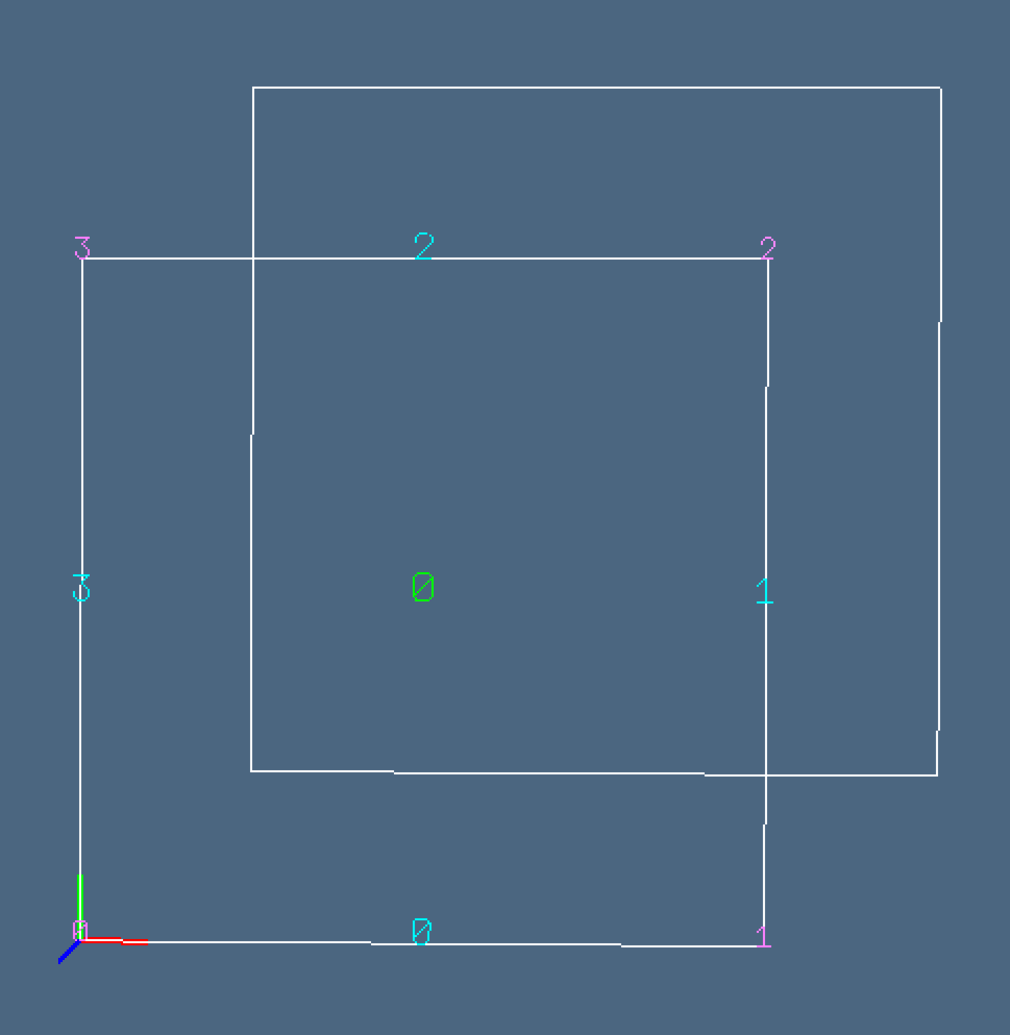
\includegraphics[height=0.325\linewidth,width=0.325\linewidth]{images/SCDC1} 
   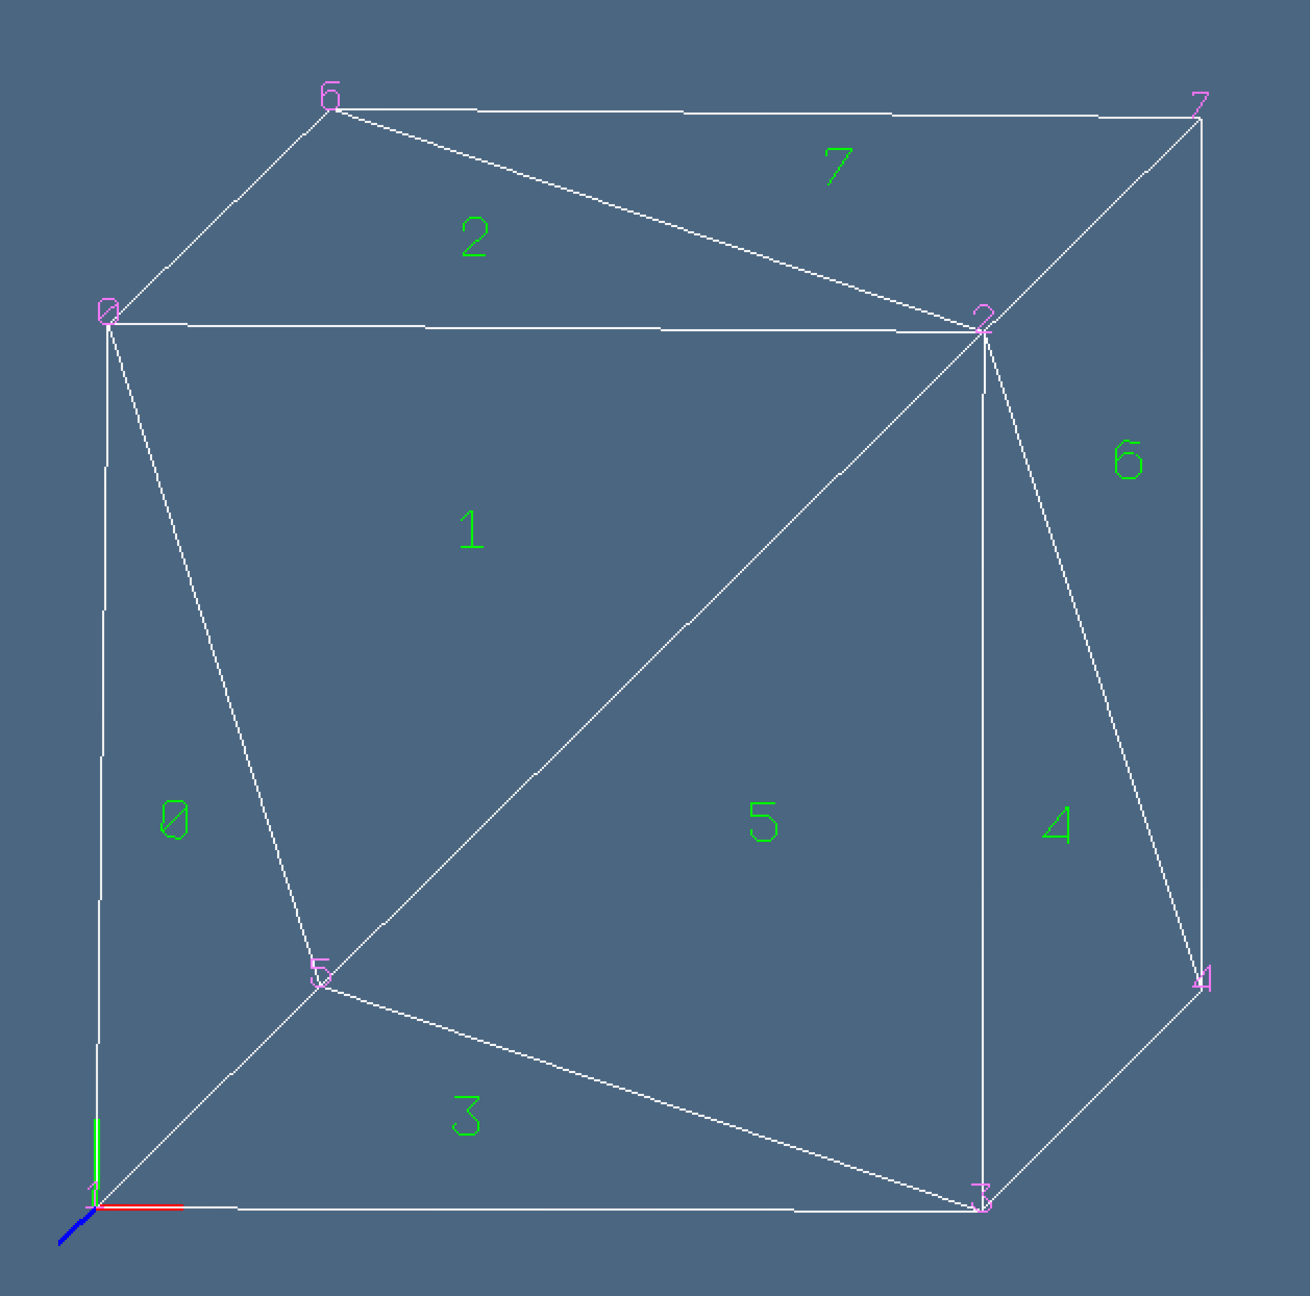
\includegraphics[height=0.325\linewidth,width=0.325\linewidth]{images/SCDC2} 
   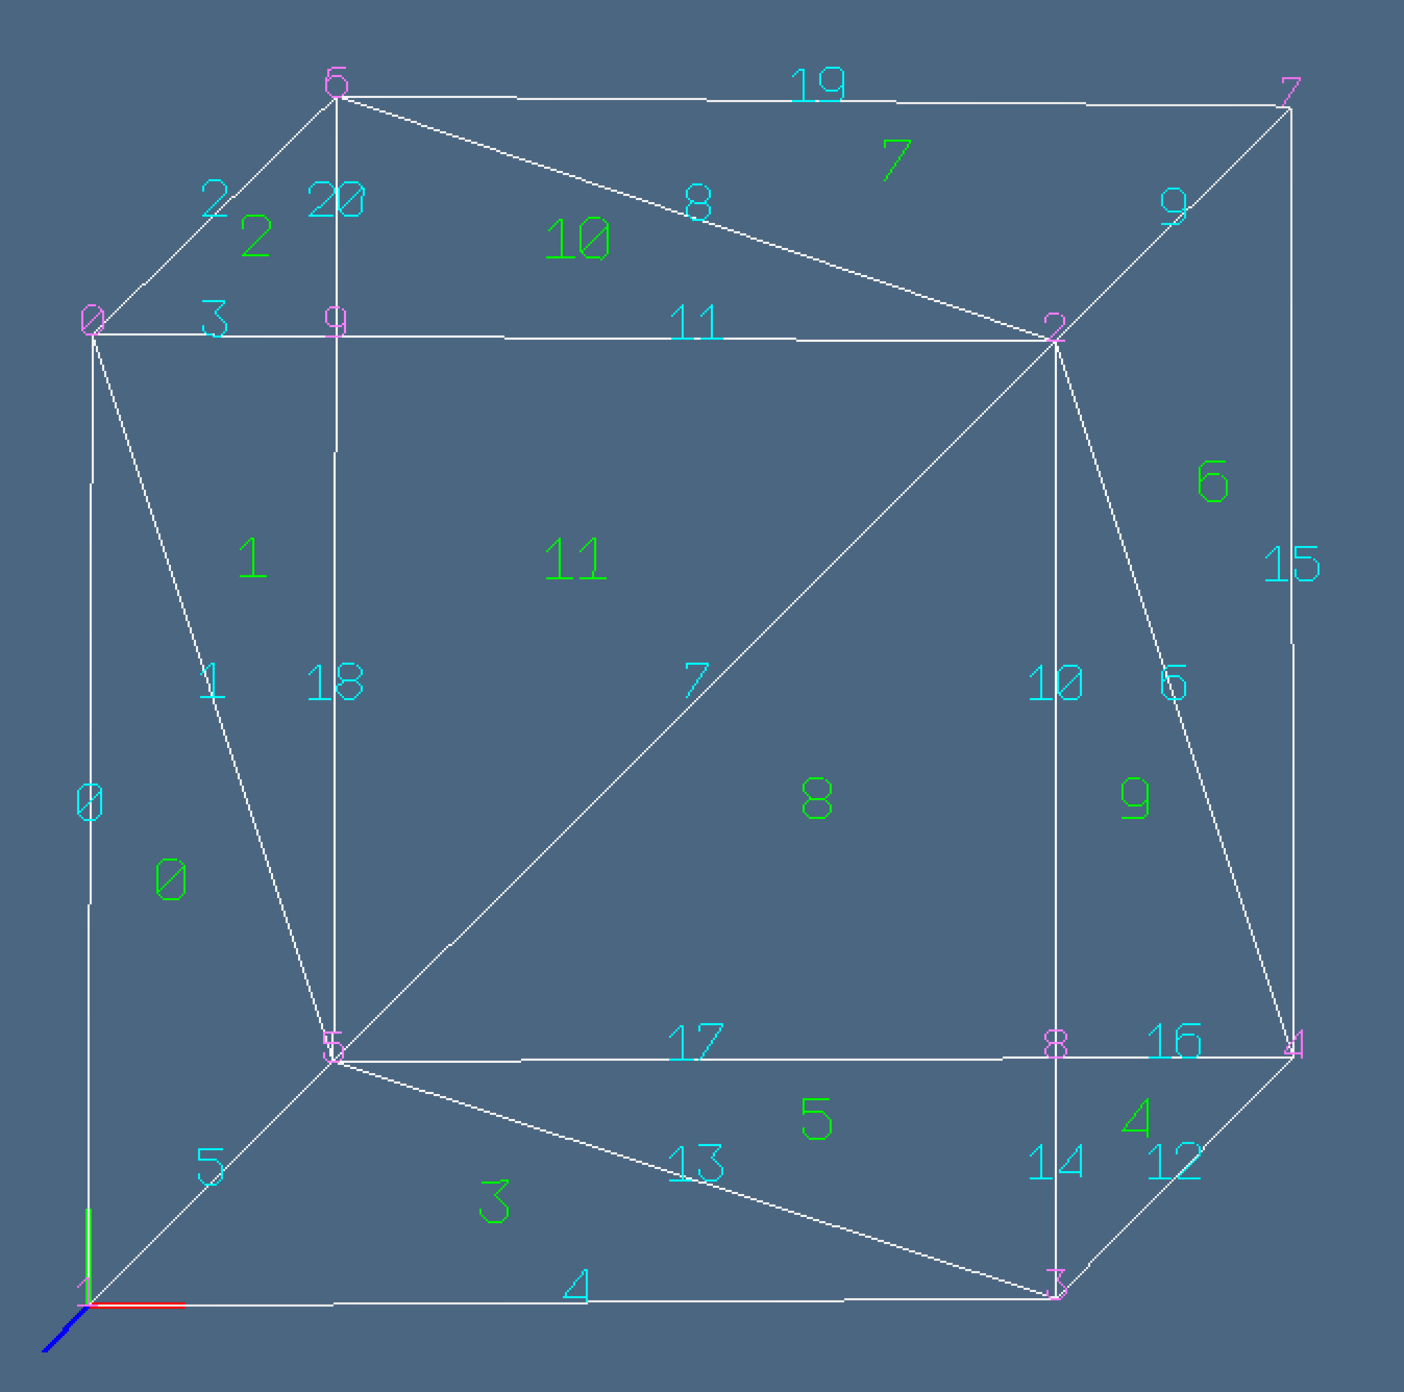
\includegraphics[height=0.325\linewidth,width=0.325\linewidth]{images/SCDC3} 
   \caption{Transformation from Boolean input (two 2D single-cell complexes) to CDC (Common Delaunay Complex) to SCDC (Split Common Delaunay Complex).}
   \label{fig:example}
\end{figure}




\section{Reconstruction of results}

Once the SCDC has been constructed, some of its $d$-cells are fully characterized, using two bits of information, as either internal (1) or external (0) to one or both the cellular spaces of Boolean arguments $A$ and $B$. 

In particular, when a CDC cell was split, the two resulting subcells were both labeled: one as internal, and the other as external to the oriented hyperplane of the splitting facet. Conversely, when such hyperplane was the support (i.e.~the affine hull) of one $(d-1)$-face of the CDC cell, just this cell was characterised as either internal or external to such support hyperplane.

A third value (-1) was used for the initial characterisation of all the SCDC cells, so that at the end of the SCDC construction, every $d$-cell is tagged with two values from the set $\{-1,0,1\}$. A recursive traversal of the cells reachable from every cell already tagged with either 0 or 1, will allow to extend the cell tag to those tagged as -1 (which stands for ``unknown position").




\subsection{Computing the coboundary of SCDC space}
\label{sec:coboundary}

The first algorithm prototype has shown that the previous tagging strategy works well in several cases, but is not sufficient in others, because the recursive extension of tags is not always correctly blocked at the boundaries of $A$ and $B$, as---of course---embedded in the SCDC. 

In this section we develop a stronger characterisation of the boundaries, by fully tagging in SCDC the internal coboundary of boundaries of $A$ and $B$. This novel strategy should allow the recursive tagging extension to work correctly in all cases.

As we know, the  coboundary operators $\delta_{k-1}: C_{k-1} \to C_k$ are the transpose of the boundary operators $\partial_k: C_k \to C_{k-1}$ ($1\leq k\leq d$). We therefore proceed to the construction of the operator $\delta_{d-1}$, according to the procedure illustrated in~\cite{}. For this purpose we need to use both the $C_d$ and the $C_{d-1}$ bases of SCDC. The first basis is generated as \texttt{CV} array during the splitting. The second basis will be built from $C_d$ using the proper $d$-adjacency algorithm from~\cite{}. 

Let us remember that a (co)boundary operator may be applied to \emph{any} chain from the linear space of chains defined upon a cellular complex. 
In our case we have already generated the $(d-1)$-chains $\partial A$ and $\partial B$ while building the SCDC, by accumulating, in the course of the splitting phase, the $(d-1)$-facets discovered while tracking the boundaries of $A$ and $B$. We just need now to tag (a subset of) $\delta_{d-1}\partial_d A$ and $\delta_{d-1}\partial_d B$.

\paragraph{Boundary triangulation of a convex hull}

The dimension-independent computation of the simplicial complex partitioning the boundary of a Delaunay triangulation is given here, using the set of \texttt{simplices} and \texttt{neighbors} provided by the \texttt{scipy.spatial} Python library using the \texttt{qhull} implementation.
It may be worth noting that the \texttt{neighbors} technique to denote the $d$-adjacencies of the simplices of a multidimensional triangulation was introduced in~\cite{DBLP:journals/cad/FerruciP91,Paoluzzi:1993:DMS:169728.169719} and in previous research reports. 

%-------------------------------------------------------------------------------
@D Boundary triangulation of a convex hull
@{""" Boundary triangulation of a convex hull """
def qhullBoundary(V):
	dim = len(V[0])
	triangulation = Delaunay(array(V))
	CV = triangulation.simplices
	Ad = triangulation.neighbors
	out = []
	for k,adjs in enumerate(Ad):
		for h in range(dim):
			if adjs[h] == -1:
				a = list(CV[k])
				a.remove(CV[k,h])
				out += [a]
	return sorted(AA(sorted)(out))
	
if __name__=="__main__":
    BV = qhullBoundary(V)
    VIEW(STRUCT(MKPOLS((V,BV))))
@}
%-------------------------------------------------------------------------------


\paragraph{Extracting a $(d-1)$-basis of SCDC}

This set of $(d-1)$-cells is needed to compute the $\partial_d$ boundary operator upon the SCDC cellular space.
Since the SCDC is a \emph{solid} complex, its intrinsic dimension equates the number of coordinates of vertices.
hence \texttt{dim = len(V[0])}. The dimension-independent algorithm implemented by the \texttt{larFacets} function
returns only the \emph{interior} $(d-1)$-cells, if the LAR of the \emph{exterior} cell(s) is not given as the last cell(s) of the \texttt{CV} array. 

Of course, for a convex complex like the SCDC, the LAR of the exterior cell coincides with that of the boundary, so that we have two possibilities: (a) compute the indices of boundary vertices (including eventually the \emph{coplanar}) using \texttt{scipy.spatial} and include their list after \texttt{CV[-1]}; (b) directly compute the $(d-1)$-cells of the boundary using the function \texttt{qhullBoundary} given below ad add them to the \texttt{larFacets} output. 

We have chosen the second option  for the sake of efficiency in the current prototype implementation. The first option will be preferred when making actual use of efficient sparse matrix techniques.

%-------------------------------------------------------------------------------
@D Extracting a $(d-1)$-basis of SCDC
@{""" Extracting a $(d-1)$-basis of SCDC """
def larConvexFacets (V,CV):
    dim = len(V[0])
    model = V,CV
    V,FV = larFacets(model,dim)
    FV = sorted(FV + qhullBoundary(V))
    return FV
    
if __name__=="__main__":
	V = [[0.0,10.0],[0.0,0.0],[10.0,10.0],[10.0,0.0],[12.5,2.5],[2.5,2.5],[2.5,12.5],
		 [12.5,12.5],[10.0,2.5],[2.5,10.0]]
	CV = [[0,1,5],[9,0,5],[9,0,6],[1,3,5],[8,4,3],[8,5,3],[2,4,7],[2,6,7],
		  [8,2,5],[8,4,2],[9,2,6],[9,2,5]]
	VV = AA(LIST)(range(len(V)))
	FV = larConvexFacets (V,CV)
	submodel = SKEL_1(STRUCT(MKPOLS((V,CV))))
	VIEW(larModelNumbering(V,[VV,FV,CV],submodel,4))
@}
%-------------------------------------------------------------------------------


\subsection{Searching for the fragmented boundaries within the SCDC}

As we already know, in order to make a partial tagging of $d$-cells of SCDC, needed for computing---using the traversal algorithm given in Section~\ref{sec:traversal}---the complete and correct tagging of all its  $d$-cells, we need to compute: (a) the matrix representation of the coboundary operator in the SCDC basis; (b) the coordinate representation, in the SCDC basis, of the split Boolean arguments. The first one is assessed in Section~\ref{sec:coboundary}; the second one is computed here.


\begin{figure}[htbp] %  figure placement: here, top, bottom, or page
   \centering
   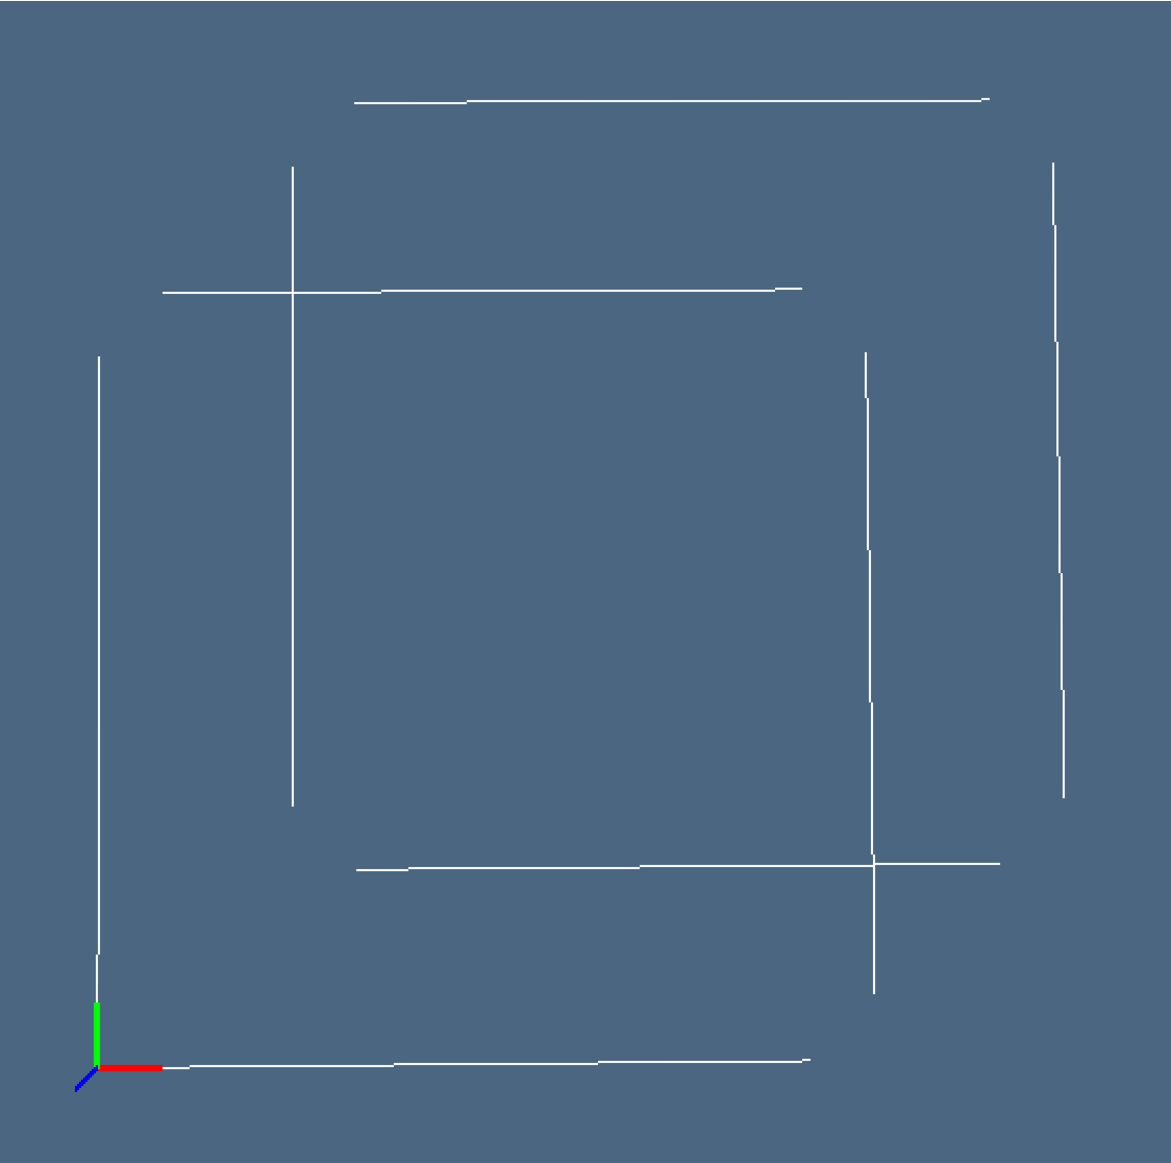
\includegraphics[height=0.325\linewidth,width=0.325\linewidth]{images/boundaryFacets1} 
   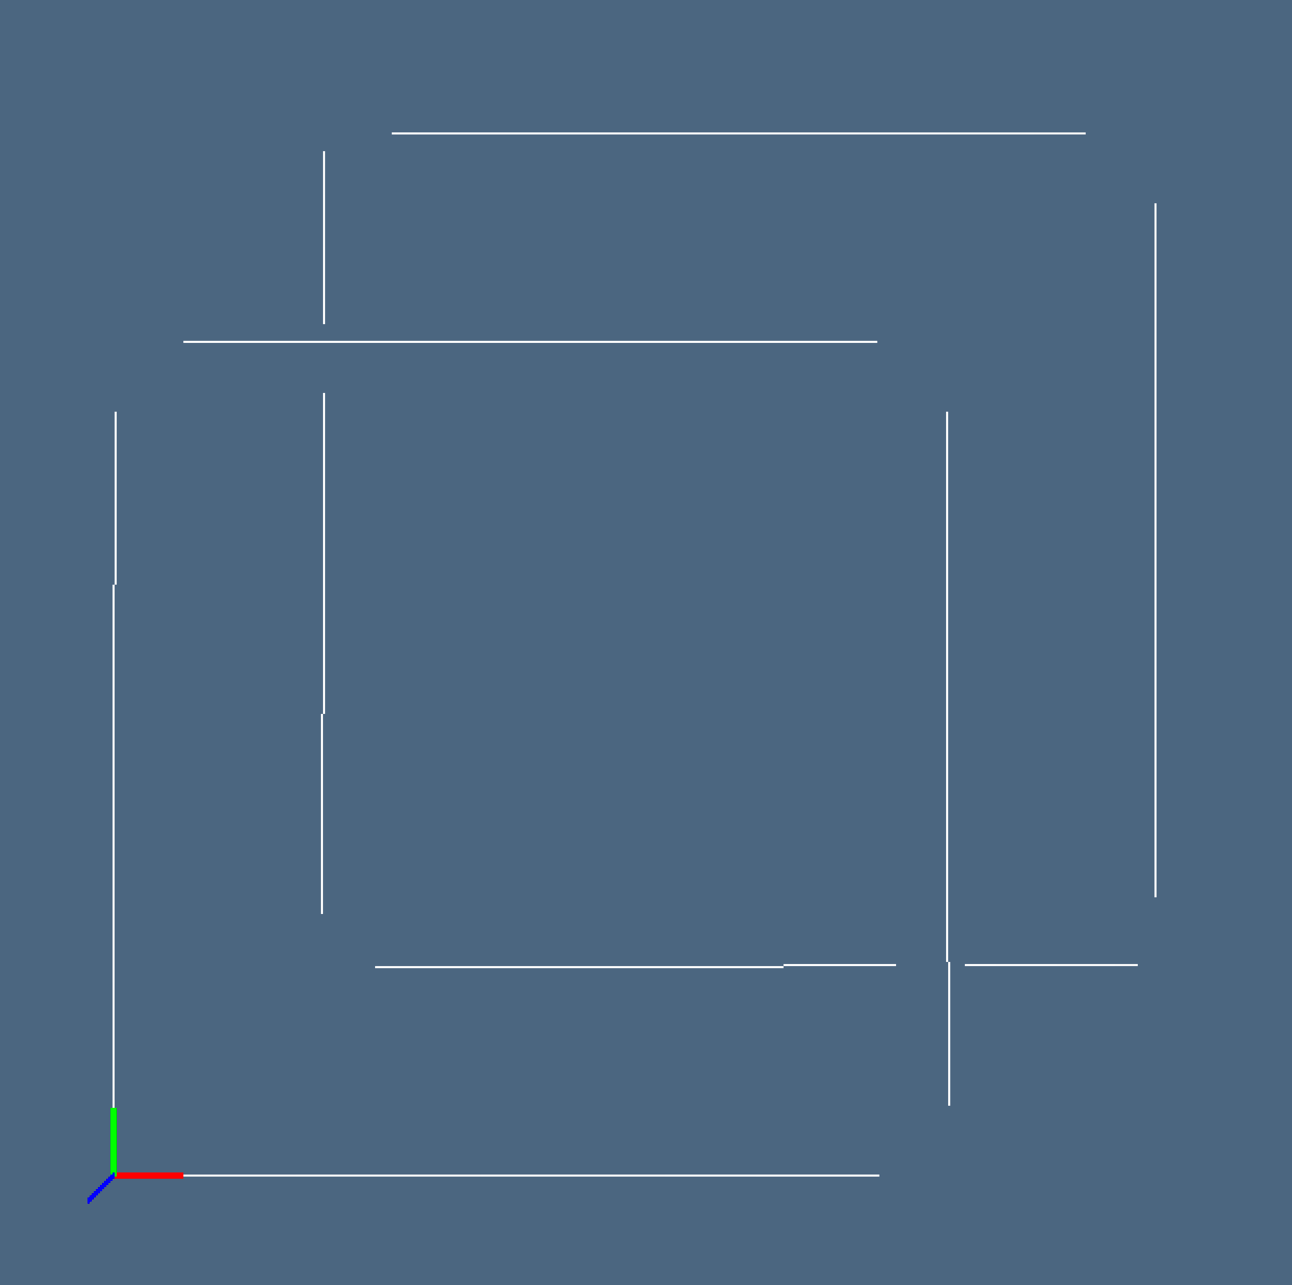
\includegraphics[height=0.325\linewidth,width=0.325\linewidth]{images/boundaryFacets2} 
   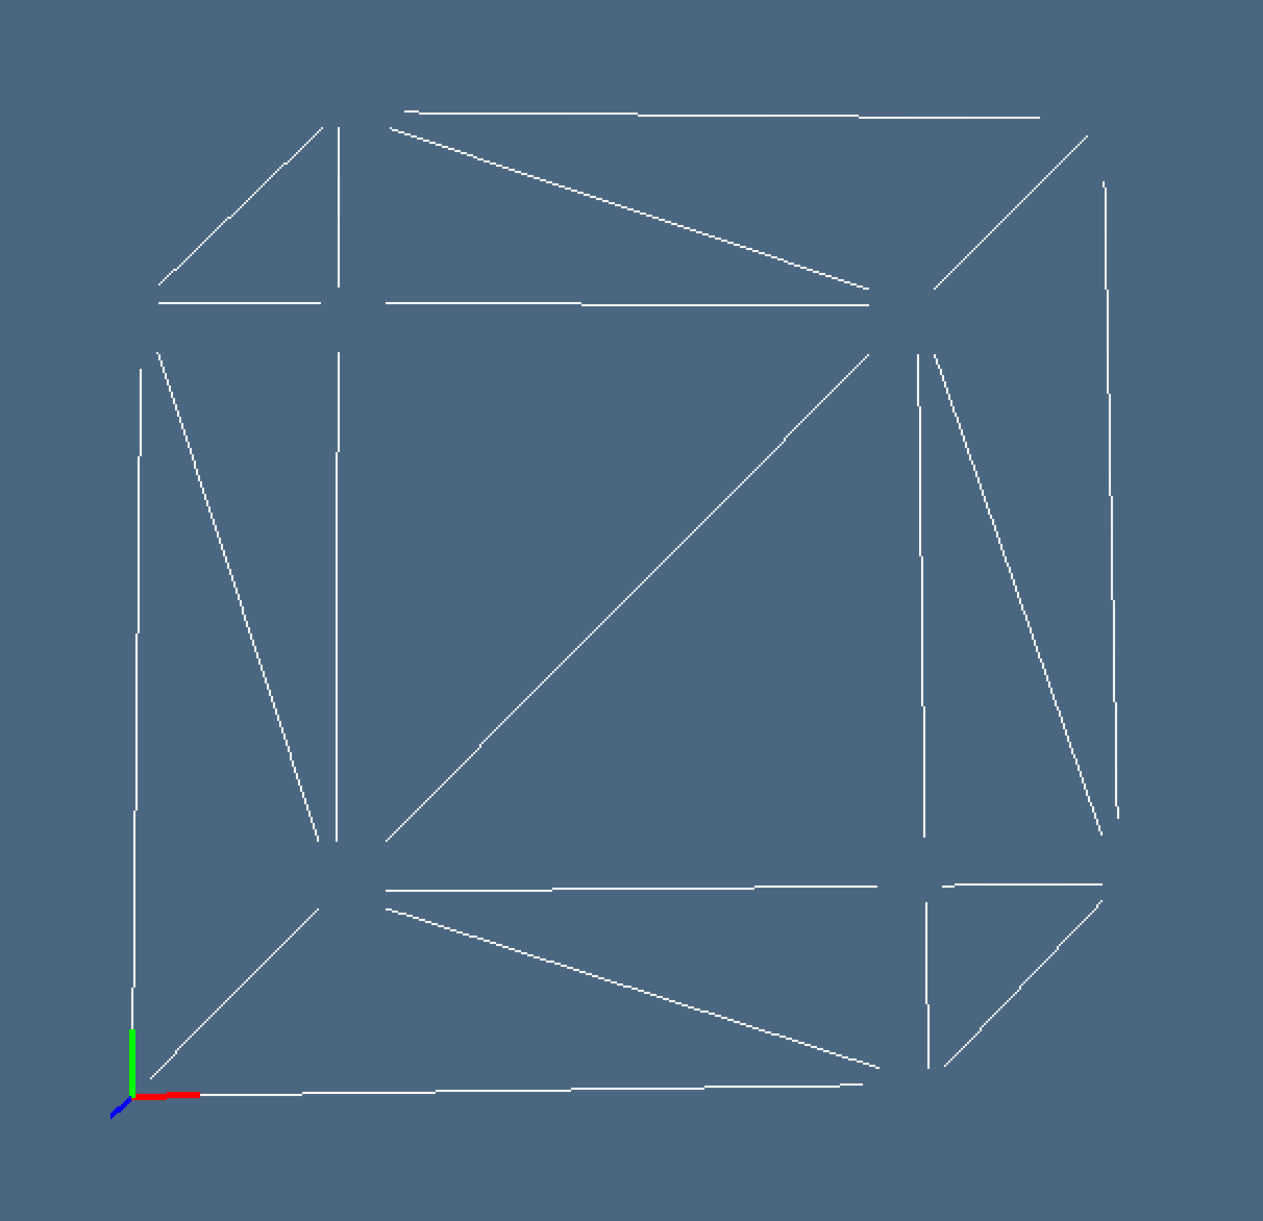
\includegraphics[height=0.325\linewidth,width=0.325\linewidth]{images/boundaryFacets3} 
   \caption{The transformation of the boundaries of two 2D Boolean arguments: (a) the $(d-1)$-cells of the input boundaries; (b) such $(d-1)$-cells accumulated during the splitting, i.e.~in intermediate phases of the SCDC construction; (c) the whole set of $(d-1)$-cells (i.e. the $(d-1)$-skeleton) of the final SCDC.}
   \label{fig:example}
\end{figure}


\paragraph{Building a dictionary of SCDC $(d-1)$-cells}
At the end of the splitting phase, the LAR model \texttt{(V,CV)} of the SCDC is built, together with a $(d-1)$-complex of accumulated split boundary cells, named \texttt{splitBoundaryFacets} in Section~\ref{sec:updating}.

%-------------------------------------------------------------------------------
@D Building a dictionary of SCDC $(d-1)$-cells
@{""" Building a dictionary of SCDC $(d-1)$-cells """
def facetBasisDict(model):
	V,CV = model
	FV = larConvexFacets (V,CV)
	values = range(len(FV))
	keys = AA(tuple)(FV)
	dict_facets = dict(zip(keys,values))
	return dict_facets

if __name__=="__main__":
	model = V,CV
	dict_facets = facetBasisDict(model)
	for cell in splitBoundaryFacets: 
		if cell in dict_facets:
			print dict_facets[cell]
		else: print cell
@}
%-------------------------------------------------------------------------------


\paragraph{Searching for the split boundary facets in the dictionary}

\paragraph{Coboundary of split boundary facets}

\paragraph{Tagging the coboundary}


\subsection{Final traversal of the SCDC}
\label{sec:traversal}

Several cells of the split CDC are tagged as either internal or external to the Boolean arguments $A$ and $B$ according to the splitting process. Such characterisation is stored within the \texttt{CVbits} array of pairs of values in $\{ -1,0,1\}$, where \texttt{CVbits[k][h]}, with $\texttt{k}\in\texttt{range(len(}C_d\texttt{))}$ and $\texttt{h}\in \texttt{range(}2\texttt{)}$, has the following meanings: 
\[
\texttt{CVbits[k][h]} = 
\begin{array}{rcl}
-1, &\quad & \mbox{if position of\ } c_k\in C_d \mbox{\ is \emph{unknown} w.r.t.~complex\ }K_h \\ 
0, &\quad & \mbox{if cell\ }c_k\in C_d \mbox{\ is \emph{external} w.r.t.~complex\ }K_h \\ 
1,  &\quad & \mbox{if cell\ }c_k\in C_d \mbox{\ is \emph{internal} w.r.t.~complex\ }K_h 
\end{array}
\]
Therefore, a double $d$-cell visit of CDC must be executed, starting from some $d$-cell interior to either $A$ or $B$, and traversing from a cell to its untraversed adjacent cells, but without crossing the complex boundary, until all cells have been visited. 

\paragraph{The initial computation of chains of Boolean arguments}

The initial setting of \texttt{CVbits[k][h]} values is done within the splitting process by the \texttt{splitCellsCreateVertices} function, and mainly by the \texttt{splittingControl} function.

\paragraph{The traversal of Boolean arguments}
Let us remember that the adjacency matrix between $d$-cells is computed via SpMSpM multiplication by the double application 
\[
\texttt{adjacencyQuery(V,CV)(cell)}, 
\] 
where the first application \texttt{adjacencyQuery(V,CV)}
returns a partial function with bufferization of the adjacentcy matrix, and the second application to \texttt{cell} returns the list of adjacent $d$-cells sharing with it a $(d-1)$-dimensional facet.

\paragraph{Traversing a Boolean argument within the CDC}
A recursive function \texttt{booleanChainTraverse} is given in the script below, where 

%-------------------------------------------------------------------------------
@D Traversing a Boolean argument within the CDC
@{""" Traversing a Boolean argument within the CDC """
def booleanChainTraverse(h,cell,V,CV,CVbits,value):
	adjCells = adjacencyQuery(V,CV)(cell)
	for adjCell in adjCells: 
		if CVbits[adjCell][h] == -1:
			CVbits[adjCell][h] = value
			CVbits = booleanChainTraverse(h,adjCell,V,CV,CVbits,value)
	return CVbits
@}
%-------------------------------------------------------------------------------


\paragraph{Input and CDC visualisation}

%-------------------------------------------------------------------------------
@D Input and CDC visualisation
@{""" Input and CDC visualisation """
submodel1 = mkSignedEdges((V1,BC1))
submodel2 = mkSignedEdges((V2,BC2))
VIEW(STRUCT([submodel1,submodel2]))
submodel = SKEL_1(STRUCT(MKPOLS((V,CV))))
VIEW(larModelNumbering(V,[VV,[],CV],submodel,4))
submodel = STRUCT([SKEL_1(STRUCT(MKPOLS((V,CV)))), COLOR(RED)(STRUCT(MKPOLS((V,BC))))])
VIEW(larModelNumbering(V,[VV,BC,CV],submodel,4))
@}
%-------------------------------------------------------------------------------


\paragraph{Boolean fragmentation and classification of CDC}

%-------------------------------------------------------------------------------
@D Boolean fragmentation and classification of CDC
@{""" Boolean fragmentation and classification of CDC """

def booleanChains(arg1,arg2):
	(V1,basis1), (V2,basis2) = arg1,arg2
	model1, model2 = (V1,basis1[-1]), (V2,basis2[-1])
	V,[VV,_,_,CV1,CV2],n12 = covering(model1,model2,2,0)
	CV = sorted(AA(sorted)(Delaunay(array(V)).simplices))
	vertdict = defaultdict(list)
	for k,v in enumerate(V): vertdict[vcode(v)] += [k]
	
	BC1 = signedCellularBoundaryCells(V1,basis1)
	BC2 = signedCellularBoundaryCells(V2,basis2)
	BC = sorted([[ vertdict[vcode(V1[v])][0] for v in cell] for cell in BC1] + [ 
			[ vertdict[vcode(V2[v])][0] for v in cell] for cell in BC2])
	BV = list(set(CAT([v for v in BC])))
	VV = AA(LIST)(range(len(V)))

	print "\n BC =",BC,'\n'

	if DEBUG: 
		@< Input and CDC visualisation @>
		
	@< New implementation of splitting dictionaries @>
	
	CVbits,cellPairs,twoCellIndices,splitBoundaryFacets = splitCellsCreateVertices( 
		vertdict,dict_fc,dict_cf,V,BC,CV,VC,len(BC1))
	showSplitting(V,cellPairs,BC,CV)
	
	@< Building a dictionary of SCDC $(d-1)$-cells @>
	dict_facets = facetBasisDict((V,CV))
	for cell in AA(tuple)(splitBoundaryFacets): 
		if cell in dict_facets:
			print dict_facets[cell]
		else: print cell
		
	VIEW(EXPLODE(1.2,1.2,1)(MKPOLS((V,larConvexFacets (V,CV)))))
	
	for cell in range(len(CV)):
		if CVbits[cell][0] == 1:
			CVbits = booleanChainTraverse(0,cell,V,CV,CVbits,1)		
		if CVbits[cell][0] == 0:
			CVbits = booleanChainTraverse(0,cell,V,CV,CVbits,0)
		if CVbits[cell][1] == 1:
			CVbits = booleanChainTraverse(1,cell,V,CV,CVbits,1)
		if CVbits[cell][1] == 0:
			CVbits = booleanChainTraverse(1,cell,V,CV,CVbits,0)
	
	chain1,chain2 = TRANS(CVbits)
	print "\ndict_cf",dict_cf
	print "\ndict_fc",dict_fc,"\n"
	return V,CV,chain1,chain2,CVbits
@}
%-------------------------------------------------------------------------------



\section{Exporting the library}


%-------------------------------------------------------------------------------
@O lib/py/bool.py
@{""" Module for Boolean ops with LAR """
DEBUG = True
from matrix import *
@< Initial import of modules @>
@< Symbolic utility to represent points as strings @>
@< Place the vertices of Boolean arguments in a common space @>
@< Building a covering of Common Delaunay Complex @>
@< Building a partition of Common Delaunay Complex of vertices @>
@< Characteristic matrix transposition @>
@< Look for cells in Delaunay, with vertices in both operands @>
@< Look for cells in cells12, with vertices on boundaries @>
@< Build intersection tasks @>
@< Trivial intersection filtering @>
@< Cell splitting @>
@< Init face-cell and cell-face dictionaries @>
@< Updating the split cell @>
@< Updating the vertex set  of split cells @>
@< Managing the splitting dictionaries @>
@< Test for split halting along a boundary facet @>
@< Computing the adjacent cells of a given cell @>
@< Show the process of CDC splitting @>
@< Boundary triangulation of a convex hull @>
@< Extracting a $(d-1)$-basis of SCDC @>
@< Traversing a Boolean argument within the CDC @>
@< Boolean fragmentation and classification of CDC @>
@}
%-------------------------------------------------------------------------------

\section{Tests}



\subsection{2D examples}

\subsubsection{First examples}

Three sets of input 2D data are prepared here, ranging from very simple to a small instance of the hardest kind of dataset, known to produce an output of size $O(n^2)$.


%-------------------------------------------------------------------------------
@D First set of 2D data: Fork-0 input
@{""" Definition of Boolean arguments """
V1 = [[3,0],[11,0], [13,10], [10,11], [8,11], [6,11], [4,11], [1,10], [4,3], [6,4], 
	[8,4], [10,3]]
FV1 = [[0,1,8,9,10,11],[1,2,11], [3,10,11], [4,5,9,10], [6,8,9], [0,7,8], [2,3,11],
	[3,4,10], [5,6,9], [6,7,8]]
EV1 = [[0,1],[0,7],[0,8],[1,2],[1,11],[2,3],[2,11],[3,4],[3,10],[3,11],[4,5],[4,10],[5,6],[5,9],[6,7],[6,8],[6,9],[7,8],[8,9],[9,10],[10,11]]
VV1 = AA(LIST)(range(len(V1)))

V2 = [[0,3],[14,2], [14,5], [14,7], [14,11], [0,8], [3,7], [3,5]]
FV2 =[[0,5,6,7], [0,1,7], [4,5,6], [2,3,6,7], [1,2,7], [3,4,6]]
EV2 = [[0,1],[0,5],[0,7],[1,2],[1,7],[2,3],[2,7],[3,4],[3,6],[4,5],[4,6],[5,6],[6,7]]
VV2 = AA(LIST)(range(len(V2)))
@}
%-------------------------------------------------------------------------------


%-------------------------------------------------------------------------------
@D First set of 2D data: Fork-1 input
@{""" Definition of Boolean arguments """
V1 = [[3,0],[11,0], [13,10], [10,11], [8,11], [6,11], [4,11], [1,10], [4,3], [6,4], 
	[8,4], [10,3]]
	
FV1 = [[0,1,8,9,10,11],[1,2,11], [3,10,11], [4,5,9,10], [6,8,9], [0,7,8]]
EV1 = [[0,1],[0,7],[0,8],[1,2],[1,11],[2,11],[3,10],[3,11],[4,5],[4,10],[5,9],[6,8],[6,9],[7,8],[8,9],[9,10],[10,11]]
VV1 = AA(LIST)(range(len(V1)))

V2 = [[0,3],[14,2], [14,5], [14,7], [14,11], [0,8], [3,7], [3,5]]
FV2 =[[0,5,6,7], [0,1,7], [4,5,6], [2,3,6,7], [1,2,7], [3,4,6]]
EV2 = [[0,1],[0,5],[0,7],[1,2],[1,7],[2,3],[2,7],[3,4],[3,6],[4,5],[4,6],[5,6],[6,7]]
VV2 = AA(LIST)(range(len(V2)))
@}
%-------------------------------------------------------------------------------


\paragraph{Input and visualisation of Boolean arguments}

%-------------------------------------------------------------------------------
@D Computation of lower-dimensional cells
@{""" Computation of edges an input visualisation """
model1 = V1,FV1
model2 = V2,FV2
basis1 = [VV1,EV1,FV1]
basis2 = [VV2,EV2,FV2]
submodel12 = STRUCT(MKPOLS((V1,EV1))+MKPOLS((V2,EV2)))
VIEW(larModelNumbering(V1,basis1,submodel12,4))
VIEW(larModelNumbering(V2,basis2,submodel12,4))
@}
%-------------------------------------------------------------------------------

\paragraph{Exporting test file}

%-------------------------------------------------------------------------------
@D Bulk of Boolean task computation
@{""" Bulk of Boolean task computation """
@< Computation of lower-dimensional cells @>

V,CV,chain1,chain2,CVbits = booleanChains((V1,basis1), (V2,basis2))
for k in range(len(CV)):  print "\nk,CVbits[k],CV[k] =",k,CVbits[k],CV[k]
if DEBUG:
	VIEW(EXPLODE(1.2,1.2,1)(MKPOLS((V,[cell for cell,c in zip(CV,chain1) if c==1] ))))
	VIEW(EXPLODE(1.2,1.2,1)(MKPOLS((V,[cell for cell,c in zip(CV,chain2) if c==1] ))))
	VIEW(EXPLODE(1.2,1.2,1)(MKPOLS((V,[cell for cell,c1,c2 in zip(CV,chain1,chain2) if c1+c2==2] ))))
	VIEW(EXPLODE(1.2,1.2,1)(MKPOLS((V,[cell for cell,c1,c2 in zip(CV,chain1,chain2) if c1+c2==1] ))))
	VIEW(EXPLODE(1.2,1.2,1)(MKPOLS((V,[cell for cell,c1,c2 in zip(CV,chain1,chain2) if c1+c2>=1] ))))
@}
%-------------------------------------------------------------------------------


%-------------------------------------------------------------------------------
@O test/py/bool/test01.py
@{
import sys
""" import modules from larcc/lib """
sys.path.insert(0, 'lib/py/')
from bool import *
@< First set of 2D data: Fork-0 input @>
@< Bulk of Boolean task computation @>
@}
%-------------------------------------------------------------------------------


\subsubsection{Two squares}




%-------------------------------------------------------------------------------
@o test/py/bool/test03.py
@{""" import modules from larcc/lib """
import sys
sys.path.insert(0, 'lib/py/')
from bool import *

V1 = [[0,0],[10,0],[10,10],[0,10]]
FV1 = [range(4)]
EV1 = [[0,1],[1,2],[2,3],[0,3]]
VV1 = AA(LIST)(range(len(V1)))

V2 = [[2.5,2.5],[12.5,2.5],[12.5,12.5],[2.5,12.5]]
FV2 = [range(4)]
EV2 = [[0,1],[1,2],[2,3],[0,3]]
VV2 = AA(LIST)(range(len(V2)))
@< Bulk of Boolean task computation @>
@}
%-------------------------------------------------------------------------------


%-------------------------------------------------------------------------------
@o test/py/bool/test04.py
@{""" import modules from larcc/lib """
import sys
sys.path.insert(0, 'lib/py/')
from bool import *

V1 = [[0,0],[10,0],[10,10],[0,10]]
FV1 = [range(4)]
EV1 = [[0,1],[1,2],[2,3],[0,3]]
VV1 = AA(LIST)(range(len(V1)))

V2 = [[2.5,2.5],[7.5,2.5],[7.5,7.5],[2.5,7.5]]
FV2 = [range(4)]
EV2 = [[0,1],[1,2],[2,3],[0,3]]
VV2 = AA(LIST)(range(len(V2)))
@< Bulk of Boolean task computation @>
@}
%-------------------------------------------------------------------------------

%-------------------------------------------------------------------------------
@o test/py/bool/test05.py
@{""" import modules from larcc/lib """
import sys
sys.path.insert(0, 'lib/py/')
from bool import *

V1 = [[2.5,2.5],[7.5,2.5],[7.5,7.5],[2.5,7.5]]
FV1 = [range(4)]
EV1 = [[0,1],[1,2],[2,3],[0,3]]
VV1 = AA(LIST)(range(len(V1)))

V2 = [[2.5,2.5],[7.5,2.5],[7.5,7.5],[2.5,7.5]]
FV2 = [range(4)]
EV2 = [[0,1],[1,2],[2,3],[0,3]]
VV2 = AA(LIST)(range(len(V2)))
@< Bulk of Boolean task computation @>
@}
%-------------------------------------------------------------------------------


\begin{figure}[htbp] %  figure placement: here, top, bottom, or page
   \centering
   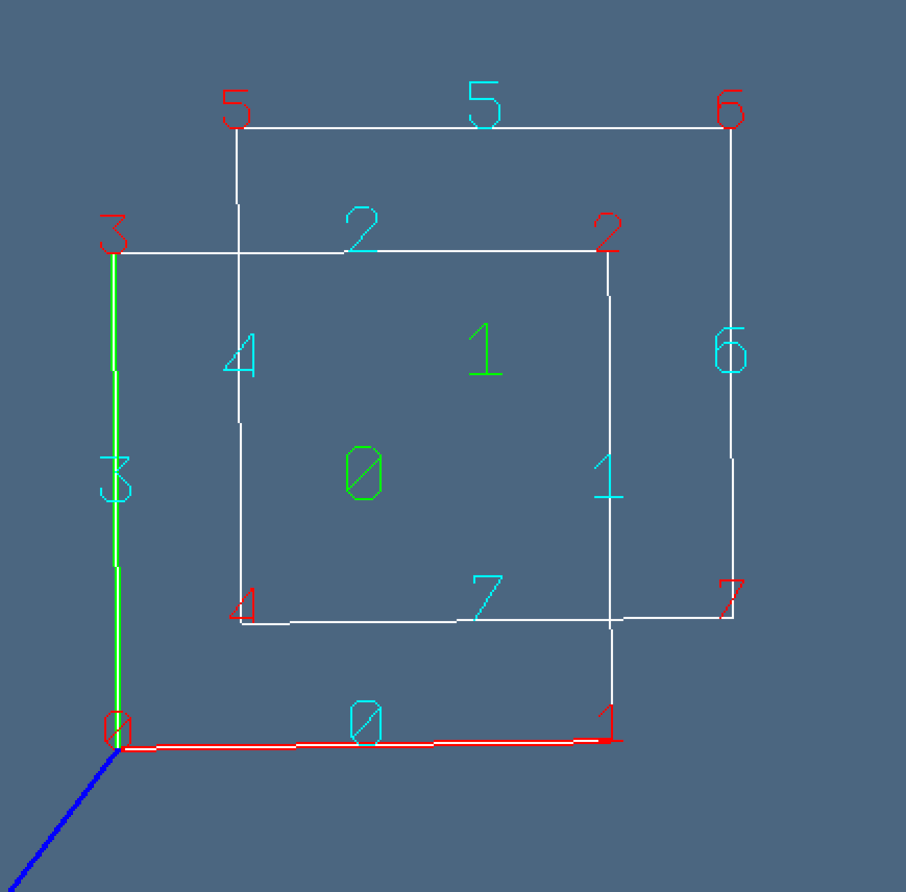
\includegraphics[height=0.244\linewidth,width=0.244\linewidth]{images/twosquares1} 
   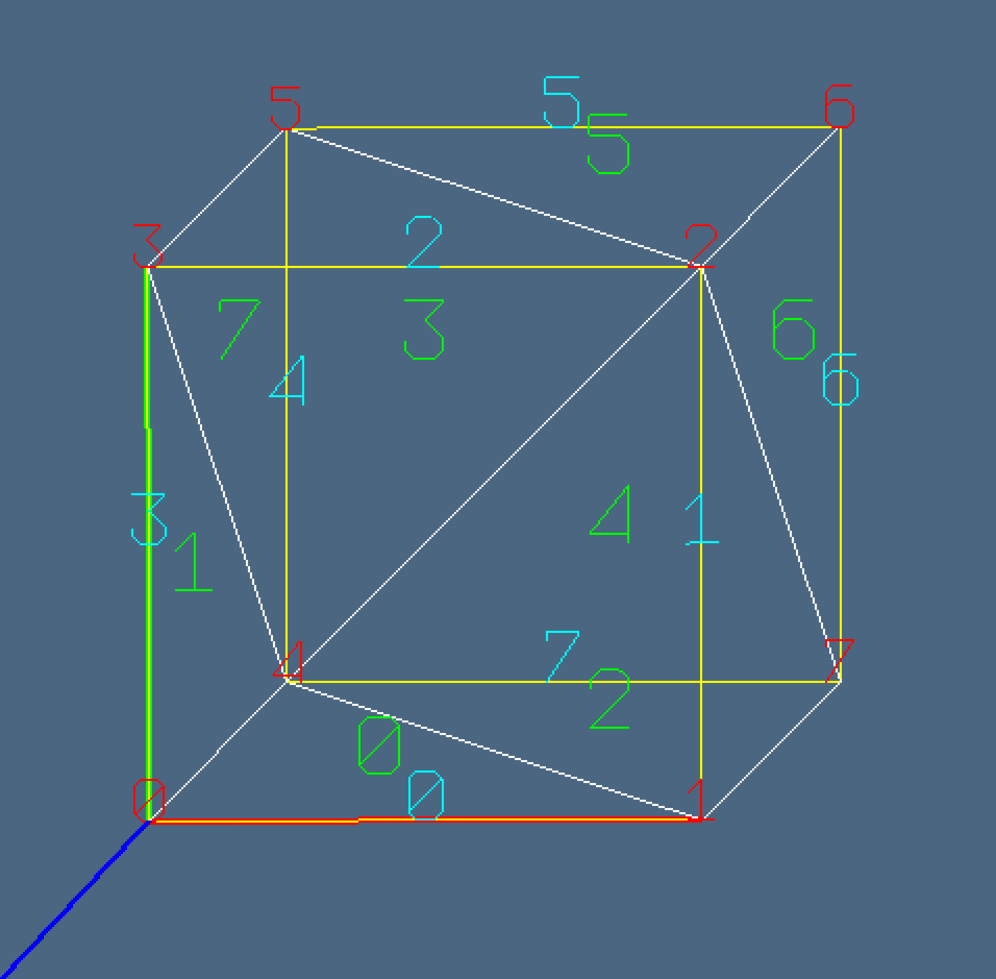
\includegraphics[height=0.244\linewidth,width=0.244\linewidth]{images/twosquares2} 
   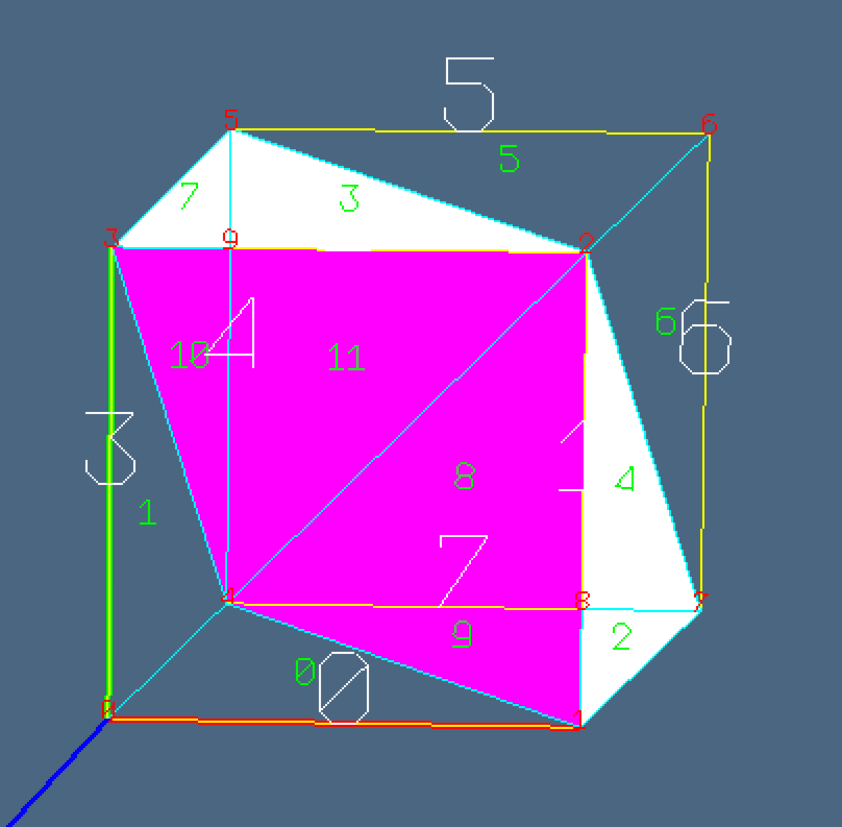
\includegraphics[height=0.244\linewidth,width=0.244\linewidth]{images/twosquares3} 
   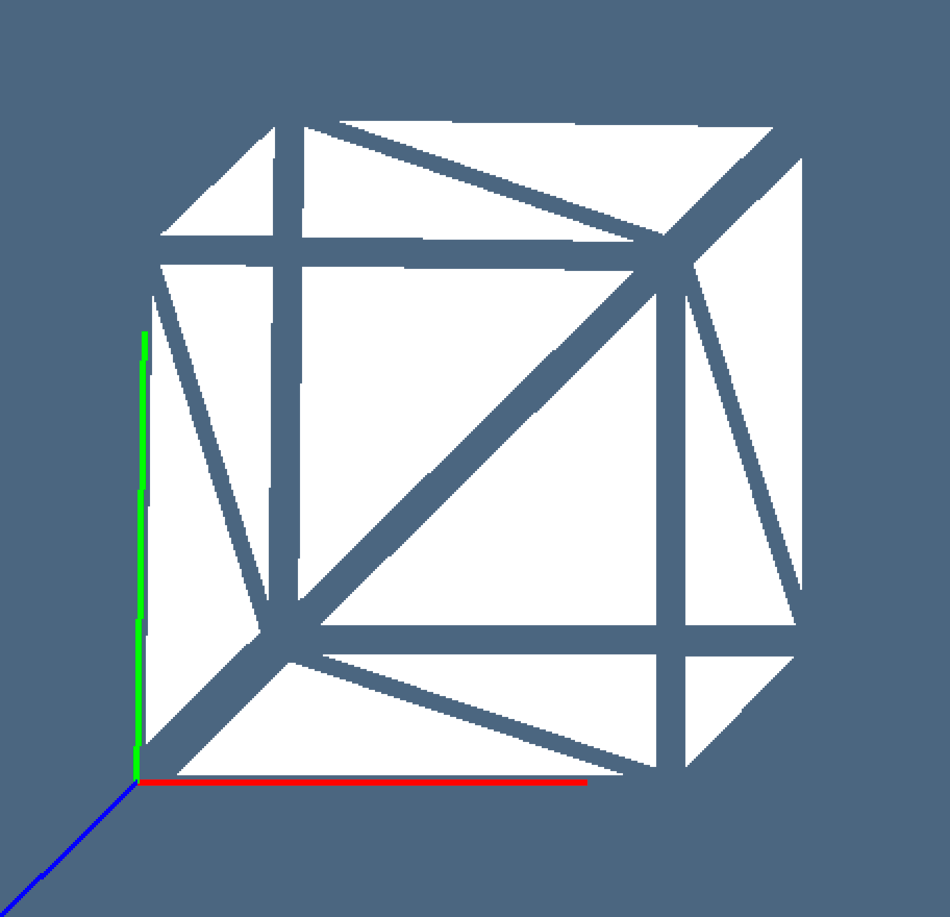
\includegraphics[height=0.244\linewidth,width=0.244\linewidth]{images/twosquares4} 
   \caption{Partitioning of the CDC (Common Delaunay Complex): (a) the two Boolean arguments merged in a single covering; (b) the CDC together with the two (yellow) boundaries; (c) the split CDC cells; (d) the exploded CDC partition.}
   \label{fig:example}
\vspace{5mm}
   \centering
   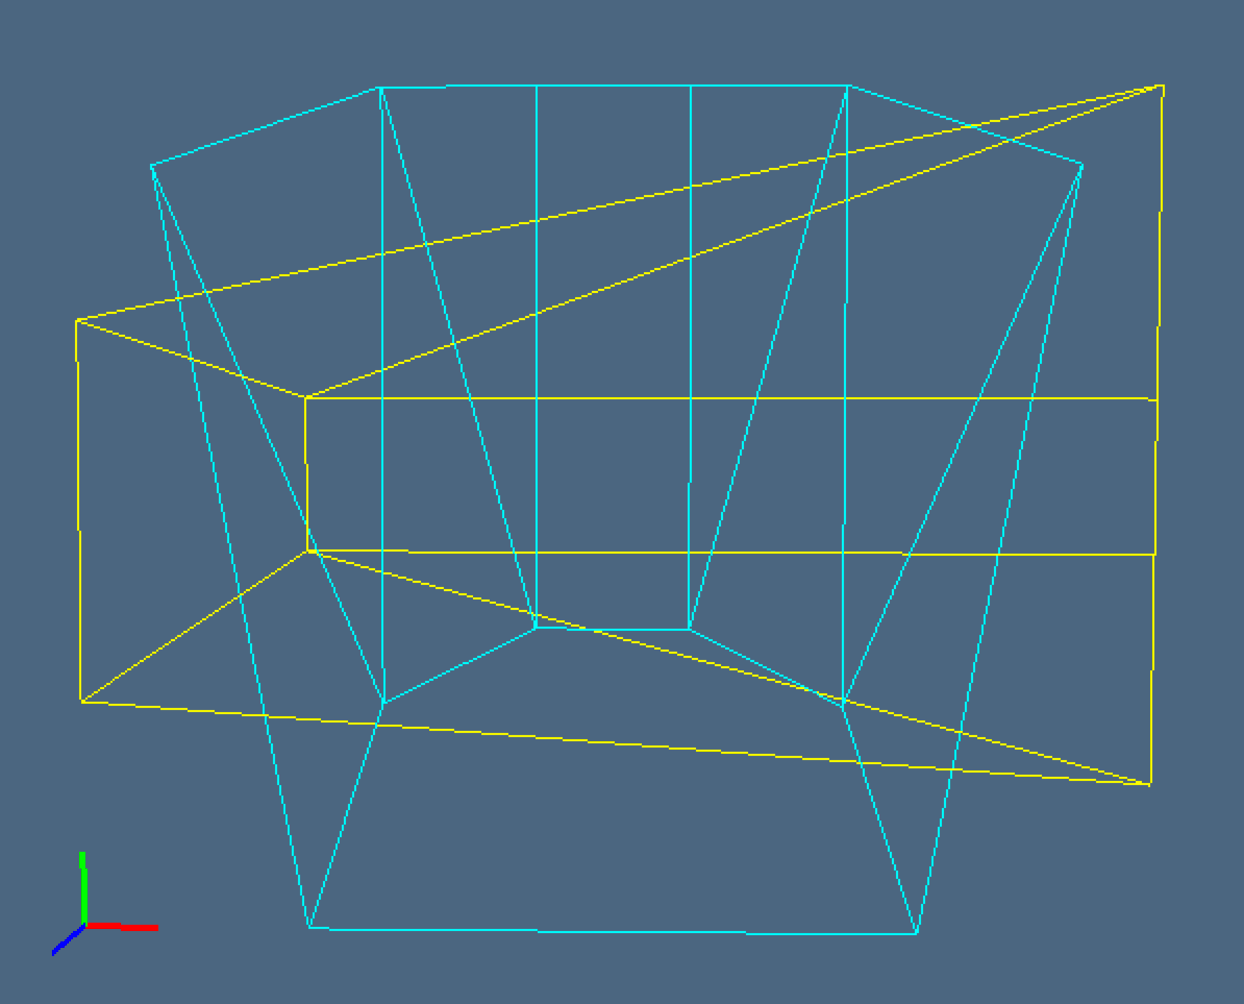
\includegraphics[height=0.2\linewidth,width=0.244\linewidth]{images/forks01} 
   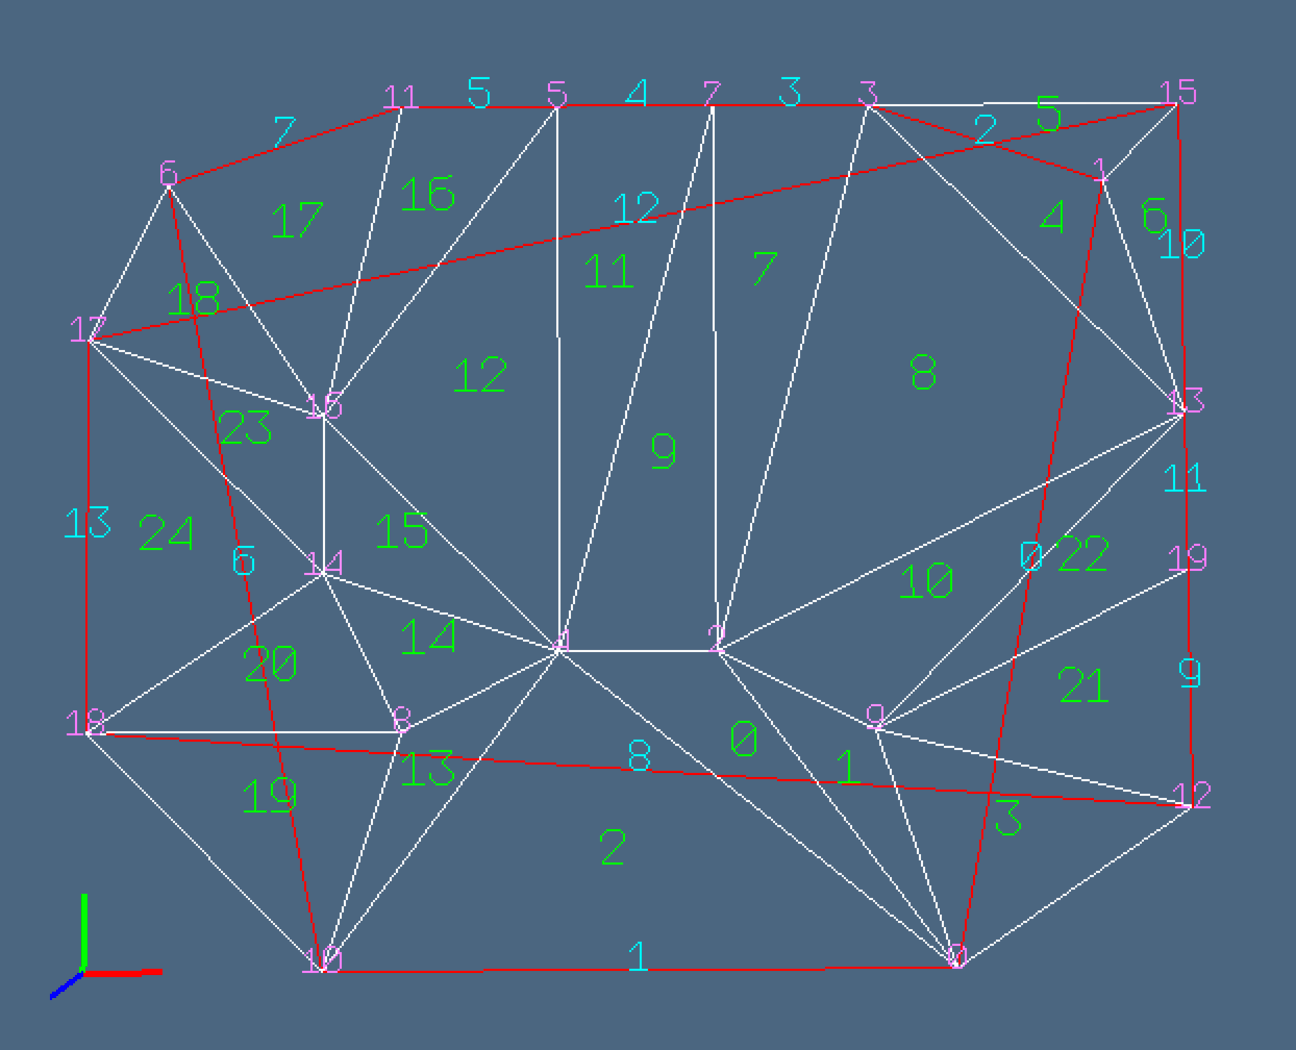
\includegraphics[height=0.2\linewidth,width=0.244\linewidth]{images/forks02} 
   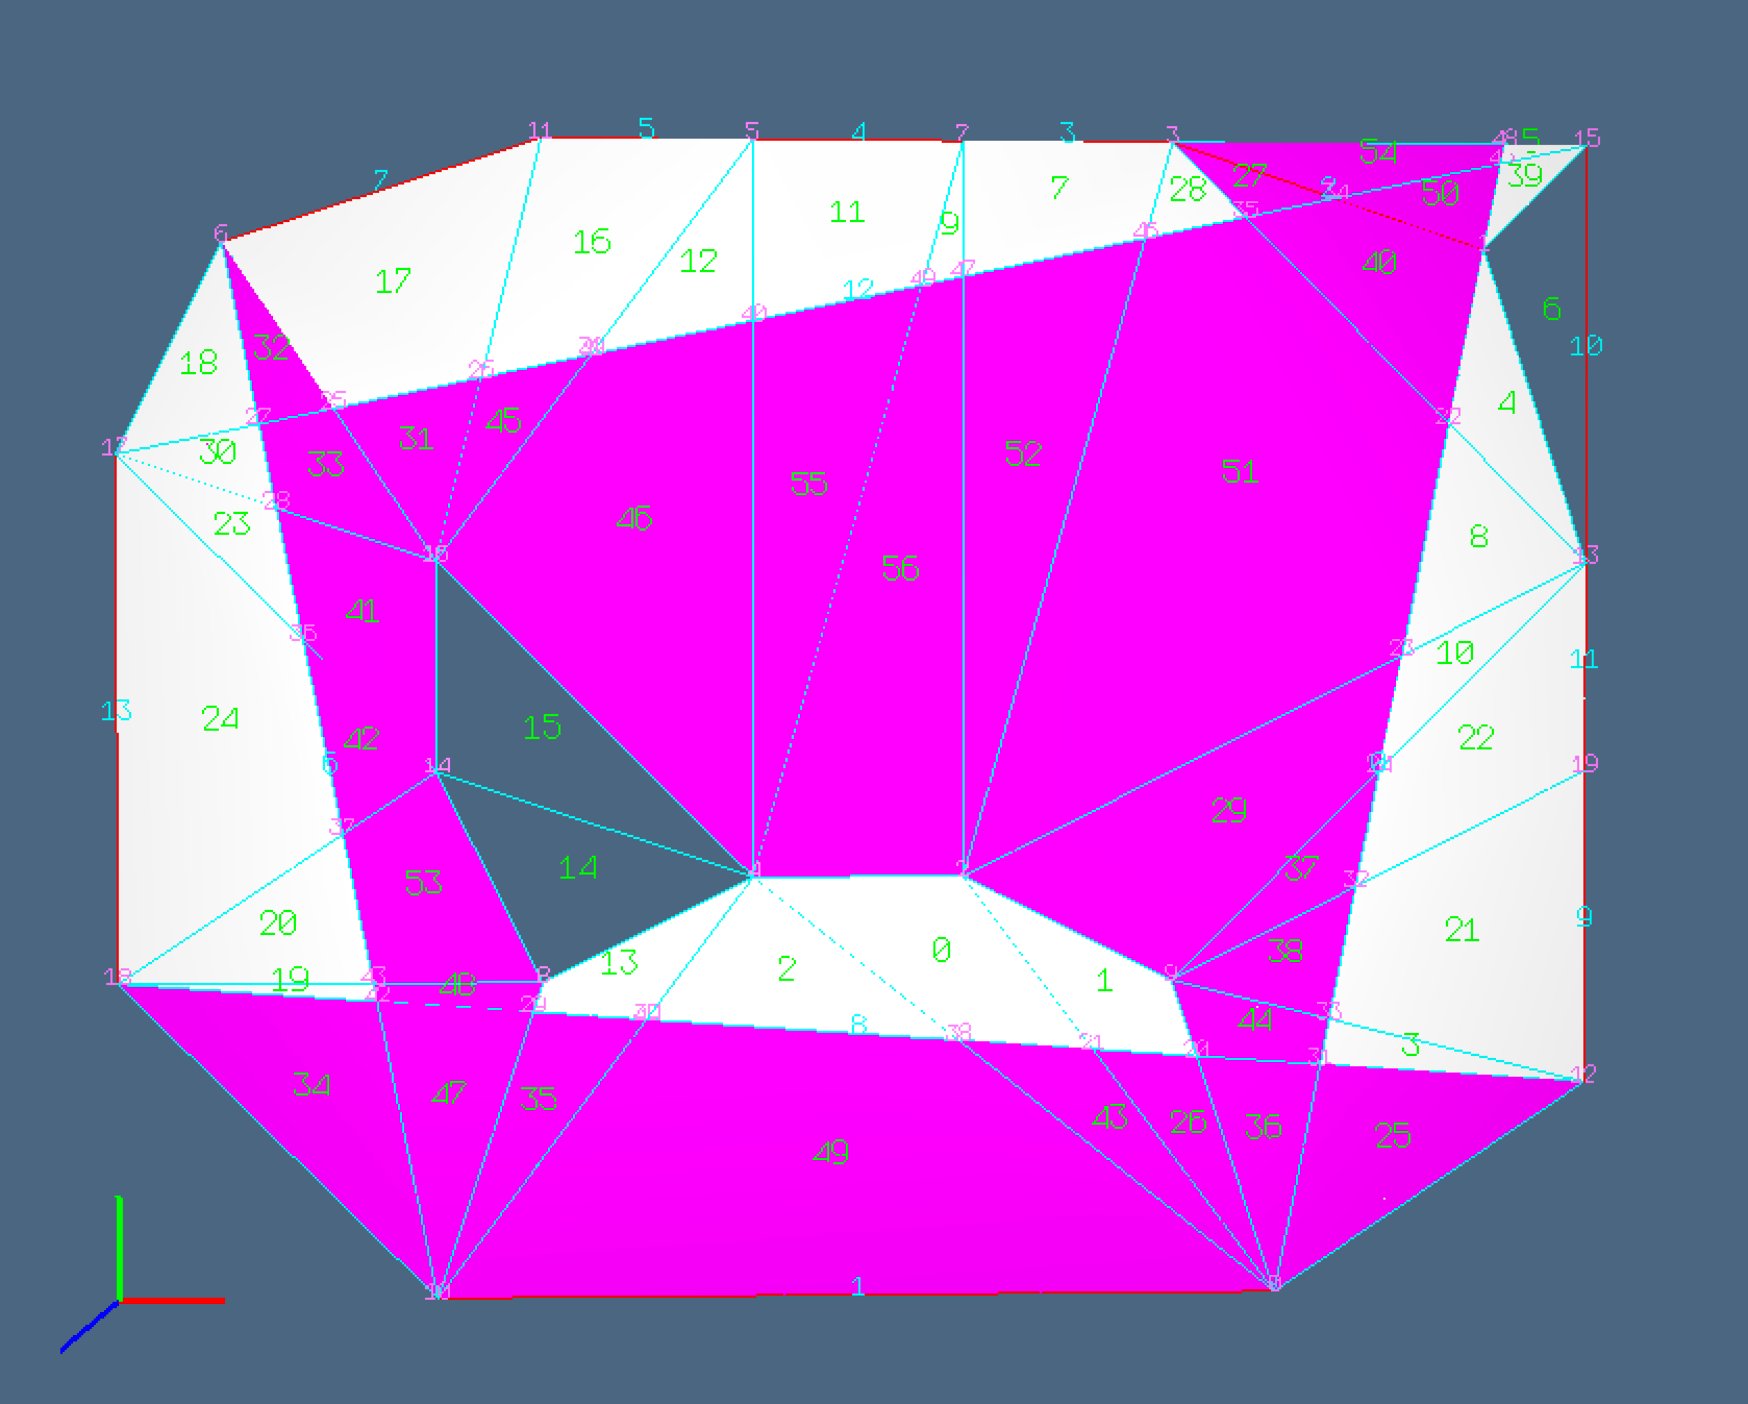
\includegraphics[height=0.2\linewidth,width=0.244\linewidth]{images/forks03} 
   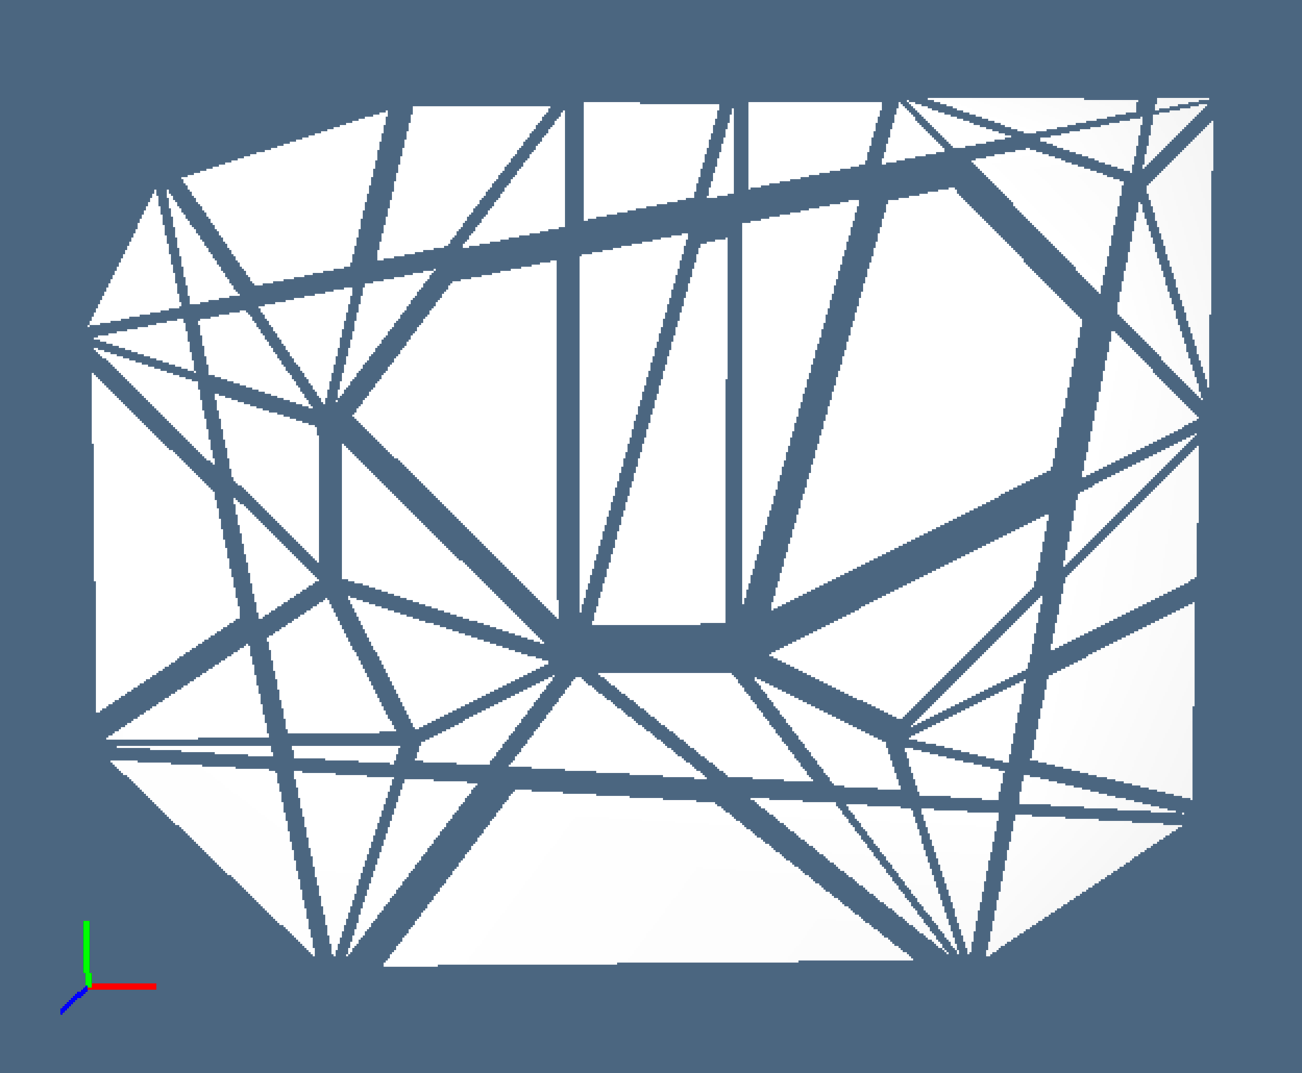
\includegraphics[height=0.2\linewidth,width=0.244\linewidth]{images/forks04} 
   \caption{Partitioning of the CDC (Common Delaunay Complex): (a) the two Boolean arguments merged in a single covering; (b) the CDC together with the two (yellow) boundaries; (c) the split CDC cells; (d) the XOR of Boolean arguments.}
   \label{fig:example}
\vspace{5mm}
   \centering
   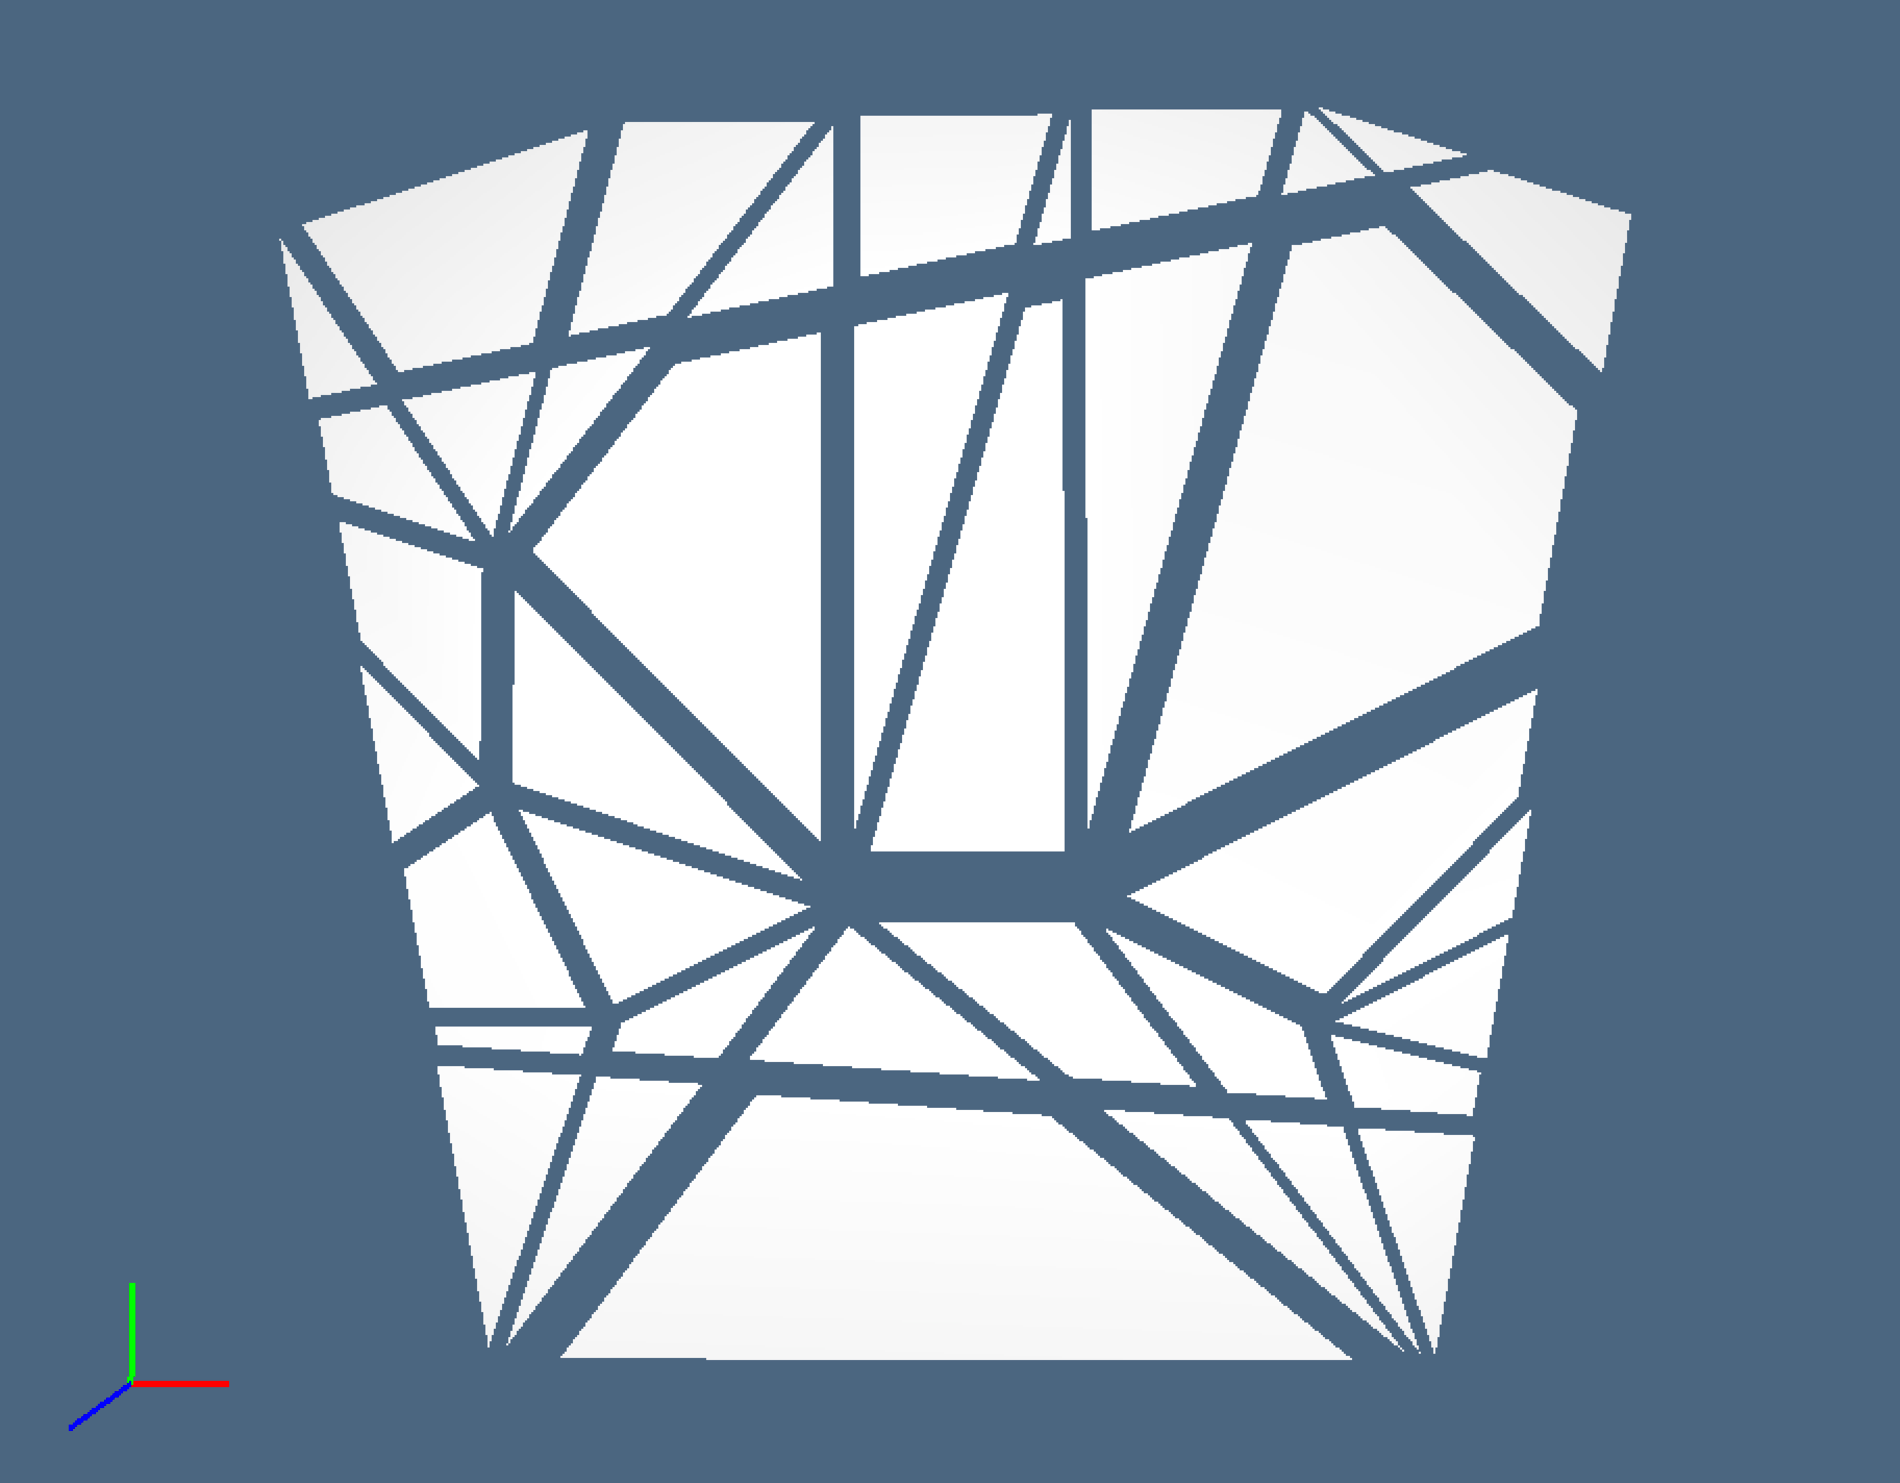
\includegraphics[height=0.2\linewidth,width=0.244\linewidth]{images/forks05} 
   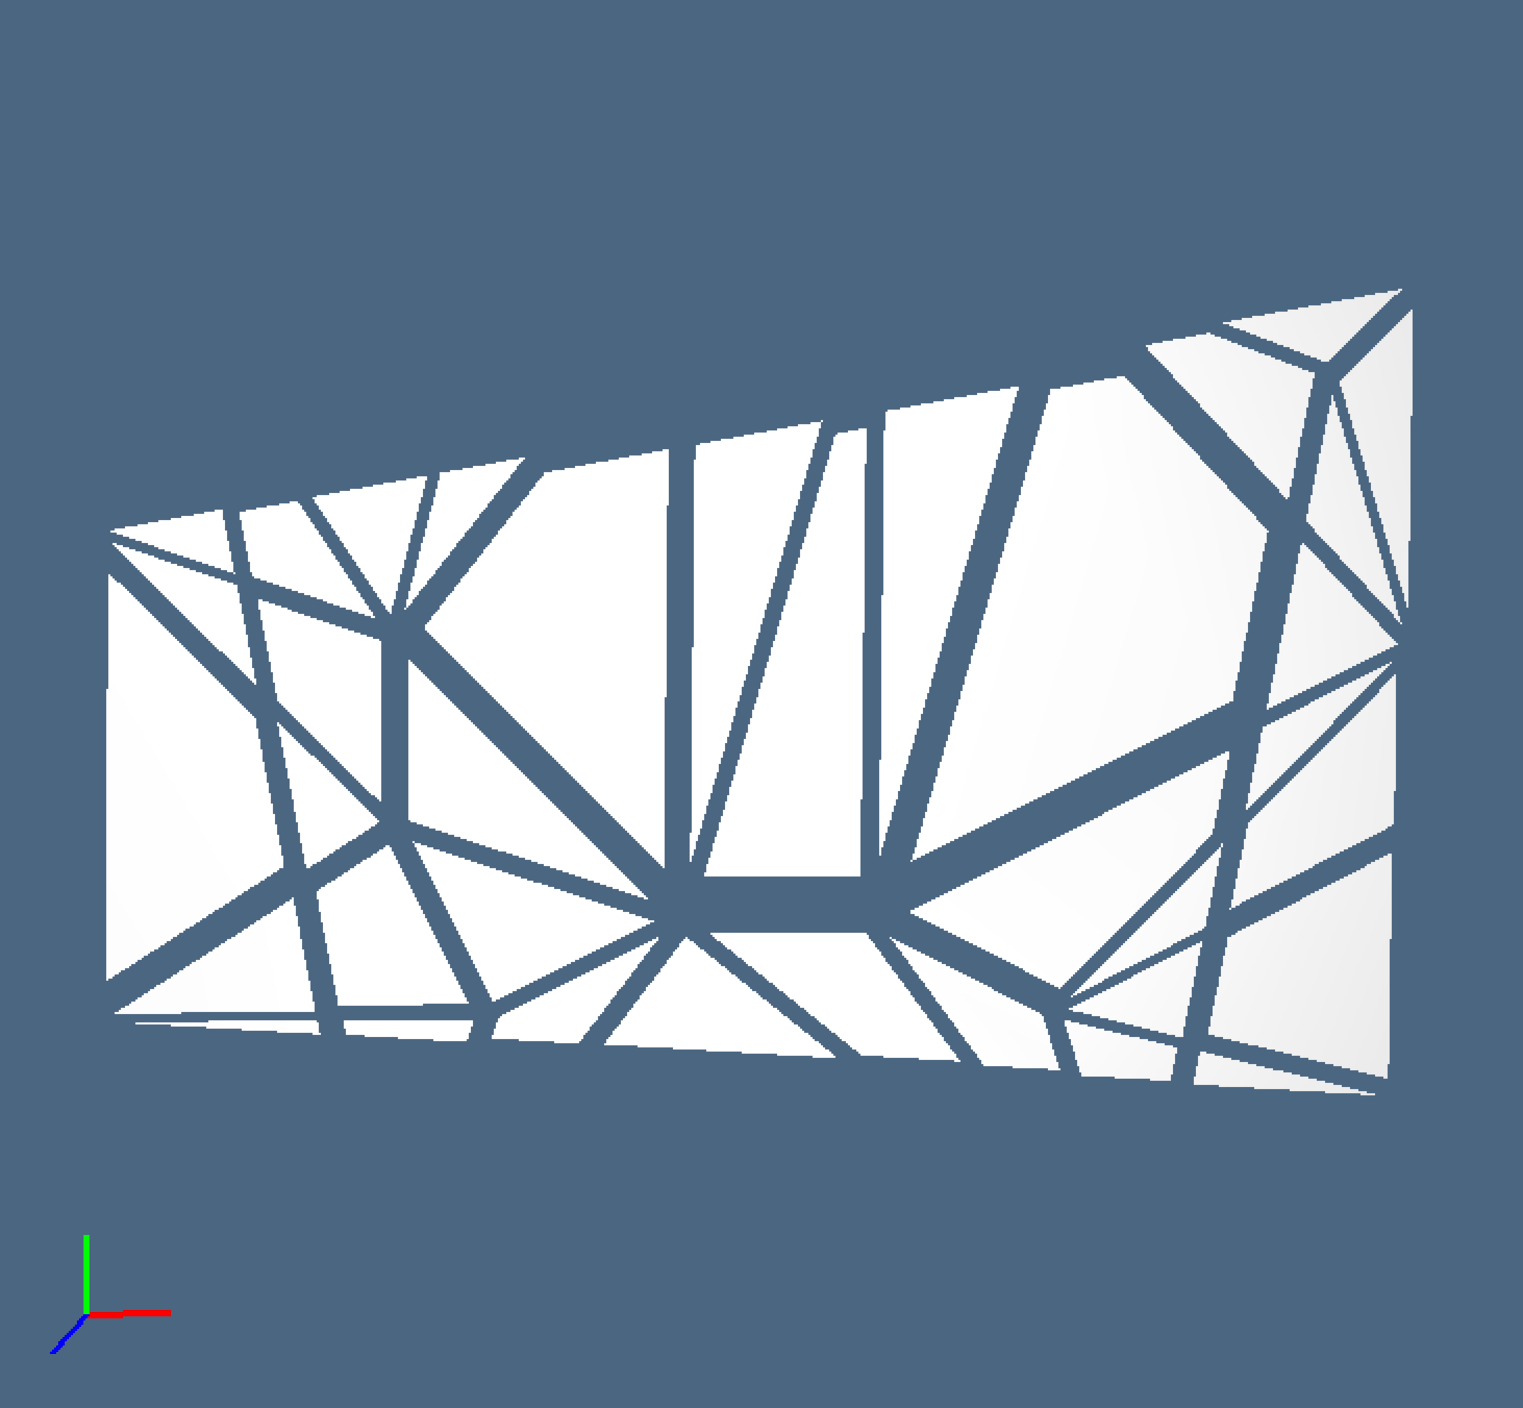
\includegraphics[height=0.2\linewidth,width=0.244\linewidth]{images/forks06} 
   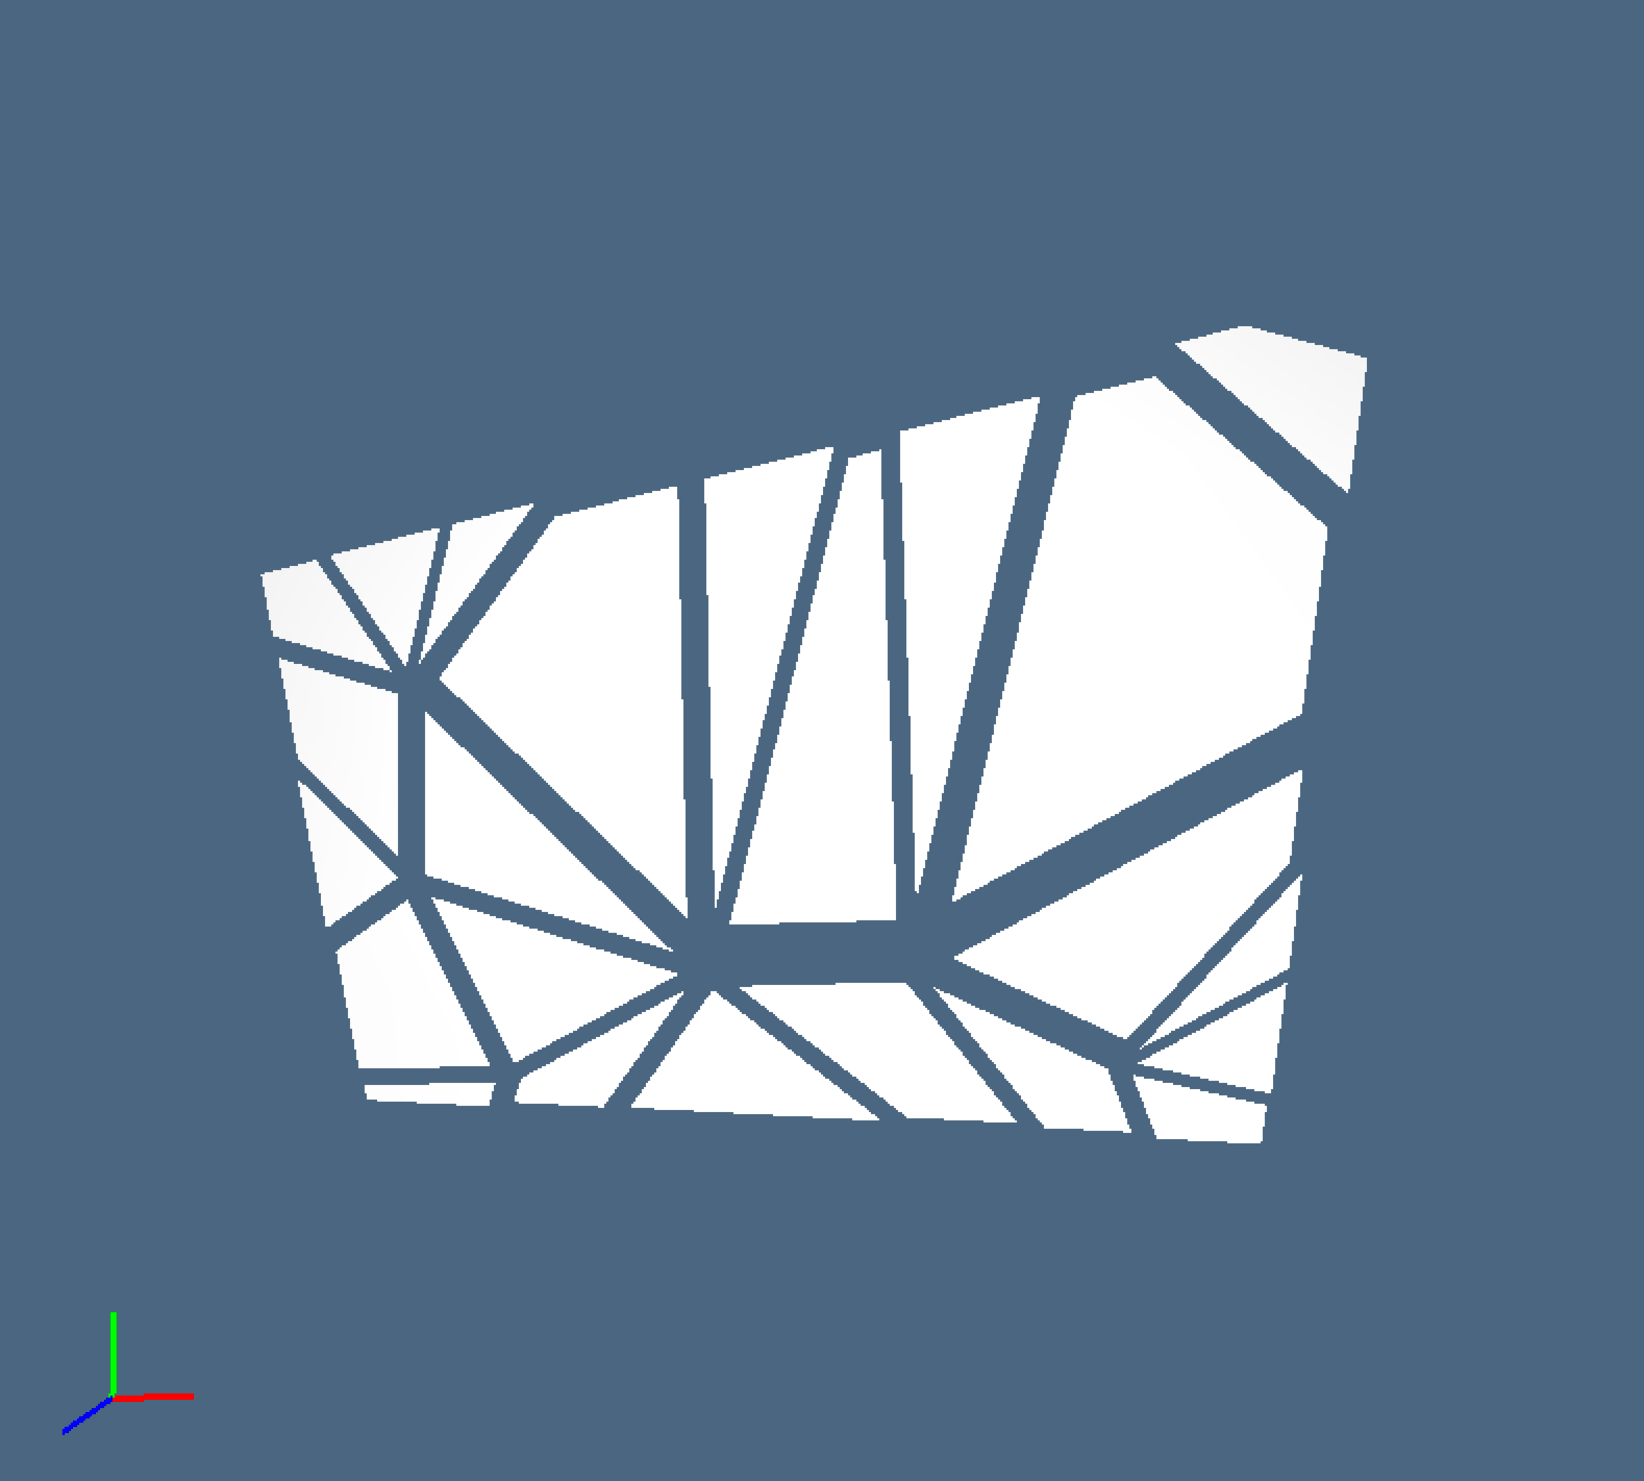
\includegraphics[height=0.2\linewidth,width=0.244\linewidth]{images/forks07} 
   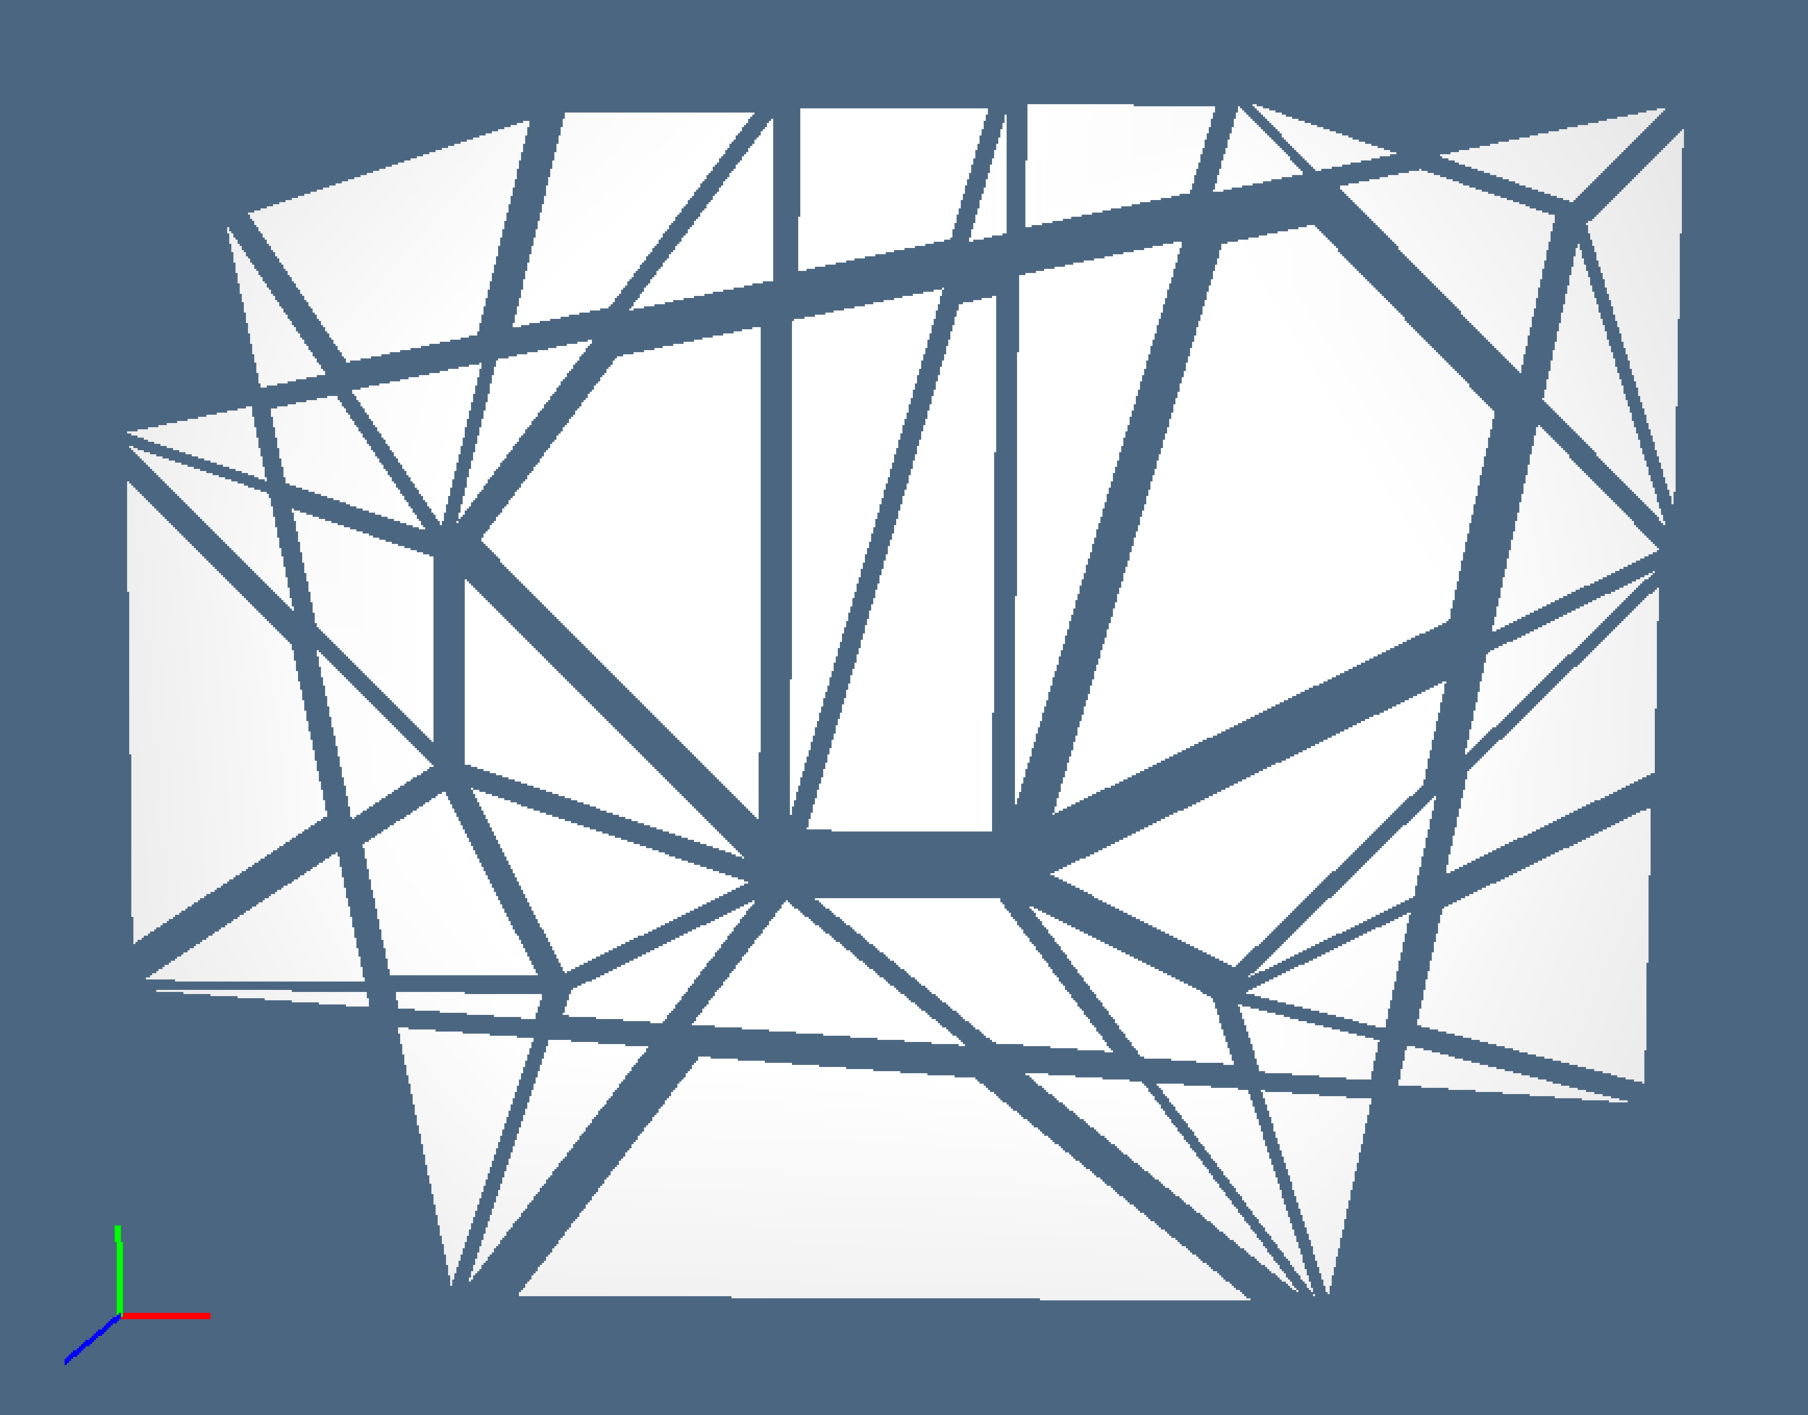
\includegraphics[height=0.2\linewidth,width=0.244\linewidth]{images/forks08} 
   \caption{Some chains defined on the CDC (Common Delaunay Complex): (a) the first Boolean argument; (b) the second Boolean argument; (c) the intersection chain; (d) the union chain.}
   \label{fig:example}
\end{figure}


%>>>>>>>>>>>>>>>>>>>>>>>>>>>>>>>>>>>>>>>>>>>>>>>>>>>>>>>>>>>>>>>>>>>>>>>>>>>>>>>
\appendix
%>>>>>>>>>>>>>>>>>>>>>>>>>>>>>>>>>>>>>>>>>>>>>>>>>>>>>>>>>>>>>>>>>>>>>>>>>>>>>>>
%-------------------------------------------------------------------------------
\section{Appendix: utility functions}
%-------------------------------------------------------------------------------
@D Initial import of modules
@{from pyplasm import *
from scipy import *
import sys
""" import modules from larcc/lib """
sys.path.insert(0, 'lib/py/')
from lar2psm import *
from simplexn import *
from larcc import *
from largrid import *
from myfont import *
from mapper import *
@}
%------------------------------------------------------------------
\subsection{Numeric utilities}

A small set of utility functions is used to transform a \emph{point} representation, given as array of coordinates, into a string of fixed format to be used as point key into python dictionaries.

%------------------------------------------------------------------
@D Symbolic utility to represent points as strings
@{""" TODO: use package Decimal (http://docs.python.org/2/library/decimal.html) """
global PRECISION
PRECISION = 3.975

def prepKey (args): return "["+", ".join(args)+"]"

def fixedPrec(value):
	out = round(value*10**PRECISION)/10**PRECISION
	if out == -0.0: out = 0.0
	return str(out)
	
def vcode (vect): 
	"""
	To generate a string representation of a number array.
	Used to generate the vertex keys in PointSet dictionary, and other similar operations.
	"""
	return prepKey(AA(fixedPrec)(vect))
@}
%------------------------------------------------------------------


\bibliographystyle{amsalpha}
\bibliography{bool}

\end{document}
